%%%%%%%%%%%%%%%%%%%%%%%%%%%%%%%%%%%%%%%%%%%%%%%%%%%%%%%%%%%%%%%%%%%%%%%%%%%%%%%
% Uni Duesseldorf
% Lehrstuhl fuer Datenbanken and Informationssysteme
% Vorlage fuer Bachelor-/Masterarbeiten
% Optimiert fuer den Original-Latex-Kompiler LATEX.EXE (LaTeX=>PS=>PDF)
% Version 1.4 - 2.3.2010
%%%%%%%%%%%%%%%%%%%%%%%%%%%%%%%%%%%%%%%%%%%%%%%%%%%%%%%%%%%%%%%%%%%%%%%%%%%%%%%

%%%%%%%%%%%%%%%%%%%%%%%%%%%%%%%%%%%%%%%%%%%%%%%%%%%%%%%%%%%%%%%%%%%%%%%%%%%%%%%
%%%%%%%%%%% BEGINN EINSTELLUNG FUER DIE ARBEIT. UNBEDINGT ERFORDERLICH! %%%%%%%
%%%%%%%%%%%%%%%%%%%%%%%%%%%%%%%%%%%%%%%%%%%%%%%%%%%%%%%%%%%%%%%%%%%%%%%%%%%%%%%
% Geben Sie Ihren Namen hier an
\newcommand{\bearbeiter}{Alina Elterman}

% Geben Sie hier den Titel Ihrer Arbeit an
\newcommand{\titel}{Metrische Dimension Spezieller Graph Klassen}

% Geben Sie das Datum des Beginns and Ende der Bachelorarbeit ein
\newcommand{\beginndatum}{28. Juni 2012}
\newcommand{\abgabedatum}{7. Dezember 2012}

% Geben Sie die Namen des Erst- and Zweitgutachters an
\newcommand{\erstgutachter}{Prof. Dr. Egon Wanke}
\newcommand{\zweitgutachter}{PD Dr. Frank Gurski}

% Falls Sie die Arbeit zweiseitig ausdrucken wollen,
% benutzen Sie die folgende Zeile mit
% \AN fuer zweiseitigen Druck
% \AUS fuer einseitigen Druck
\newcommand{\zweiseitig}{\AUS}

% Falls die Arbeit in englischer Sprache verfasst 
% werden soll, dann benutzen Sie die folgende Zeile mit
% englisch fuer englische Sprache
% deutsch fuer deutsche Sprache
\newcommand{\sprache}{deutsch}
%%%%%%%%%%%%%%%%%%%%%%%%%%%%%%%%%%%%%%%%%%%%%%%%%%%%%%%%%%%%%%%%%%%%%%%%%%%%%%%%%
%%%%%%%%%%%%%%%%%%%%%%%%%%%%%%% ENDE EINSTELLUNGEN %%%%%%%%%%%%%%%%%%%%%%%%%%%%%%
%%%%%%%%%%%%%%%%%%%%%%%%%%%%%%%%%%%%%%%%%%%%%%%%%%%%%%%%%%%%%%%%%%%%%%%%%%%%%%%%%

% Die folgende Zeile NICHT EDITIEREN oder loeschen
% (Zum Ab�ndern der BA-Vorlage in eine MA-Vorlage muessen sie
% jedoch die Datei titelmakros1.tex selbst editieren.)
%%%%%%%%%%%%%%%%%%%%%%%%%%%%%%%%%%%%%%%%%%%%%%%%%%%%%%%%%%%
% Obere Titelmakros. Editieren Sie diese Datei nur, wenn
% Sie sich ABSOLUT sicher sind, was Sie da tun!!!
% (Z.B. zum Abaendern der BA-Vorlage in eine MA-Vorlage)
% Uni Duesseldorf
% Lehrstuhl fuer Datenbanken und Informationssysteme
% Version 2.2 - 2.3.2010
%%%%%%%%%%%%%%%%%%%%%%%%%%%%%%%%%%%%%%%%%%%%%%%%%%%%%%%%%%%
\newcommand{\AN}{twoside}
\newcommand{\AUS}{}
%\newcommand{\englisch}{}
%\newcommand{\deutsch}{\usepackage[german]{babel}}

%% Die folgenden auskommentierten Optionen dienen der automatischen
%% Erkennung des Latex-Kompilers und dem Setzen der davon abh�ngigen
%% Einstellungen. Bei Problem z.B. mit dem Einbinden von verschiedenen
%% Grafiktypen bei Verwendung von PdfLatex oder Latex, einfach die
%% verschiedenen \usepackage(s) ausprobieren. (Mit diesen Einstellungen
%% funktionierte diese Vorlage bei der Verwenundg von latex.exe als
%% Kompiler bei den meisten Studierenden.)

%\newif\ifpdf \ifx\pdfoutput\undefined
%\pdffalse % we are not running pdflatex
%\else
%\pdfoutput=1 % we are running pdflatex
%\pdfcompresslevel=9 % compression level for text and image;
%\pdftrue \fi[cleardoublepage=plain]

\documentclass[11pt,a4paper,pointlessnumbers, \zweiseitig]{scrreprt}



%\usepackage[iso]{umlaute}
%\usepackage[latin1]{inputenc}
\usepackage{palatino} % palatino Schriftart
%\usepackage{makeidx} % um ein Index zu erstellen
\usepackage{tocbibind}
\usepackage[T1]{fontenc} %fuer richtige Trennung bei Umlauten
\usepackage{fancybox} % fuer die Rahmen
\usepackage{shortvrb}
\usepackage{ifthen}
%\ifthenelse{\equal{\sprache}{deutsch}}{\usepackage[ngerman]{babel}}{}
\usepackage[utf8]{inputenc}
\usepackage[ngerman]{babel}
\usepackage{lmodern} 
\usepackage{amsmath}
\usepackage{oldgerm}
\usepackage{amssymb}
\usepackage{pdfpages}
\usepackage{hyperref}
%\usepackage{fancyheadings}
\usepackage{fancyhdr}
\usepackage{amsfonts}
%\usepackage{complexity}
\usepackage{amsthm}
\usepackage{color}
\usepackage{caption}
%\usepackage{stmaryrd}
\usepackage{graphicx}
\usepackage{graphics}
\usepackage{nomencl}
\usepackage[normalem]{ulem} 
\usepackage{verbatim}
\usepackage{ulsy}
\usepackage{floatflt}
\usepackage{float}
\usepackage{tikz}
\usepackage{pgf}
\usepackage{bbding}
\usepackage{nicefrac}
\usepackage{stmaryrd}
\usepackage{tabularx}
\usepackage{multirow}
\usepackage{array}
\usepackage{algorithm}
\usepackage{algorithmic}
% \usepackage[disable]{todonotes}				% alle todo-Anmerkungen ausblenden
\usepackage[german, color=yellow!40, colorinlistoftodos, textsize=footnotesize, shadow]{todonotes}
\usetikzlibrary{arrows,automata,petri,shapes,snakes}


\newcommand{\markup}[1]{\uline{#1}}
% Befehl umbenennen in abk
\let\abk\nomenclature

\usepackage{a4wide} % ganze A4 Weite verwenden

%\ifpdf
%\usepackage[pdftex,xdvi]{graphicx}
%\usepackage{thumbpdf} %thumbs fuer Pdf
%\usepackage[pdfstartview=FitV]{hyperref} %anklickbares Inhaltsverzeichnis
%\else
%\usepackage[dvips,xdvi]{graphicx}
%\usepackage{hyperref} %anklickbares Inhaltsverzeichnis
%\fi

%%%%%%%%%%%%%%%%%%%%%%% Massangaben fuer die Arbeit %%%%%%%%%%%%%%%
\setlength{\textwidth}{15cm}

\setlength{\oddsidemargin}{35mm}
\setlength{\evensidemargin}{25mm}

\addtolength{\oddsidemargin}{-1in}
\addtolength{\evensidemargin}{-1in}

%\makeindex
% Umgebungen f"ur S�tze usw.
\clearpage{\pagestyle{empty}\cleardoublepage}
\newtheorem{bem}{Bemerkung}
\newtheorem{definition}{Definition}
\newtheorem{bezeichnungen}{Bezeichnungen}
\newtheorem{fakt}{Fakt}
\newtheorem{beispiel}{Beispiel}
\newtheorem{bsp}{Beispiel}
\newtheorem{satz}{Satz}
\newtheorem{lem}{Lemma}
\newtheorem{folg}{Folgerung}
\newtheorem{idee}{Idee}
\newtheorem{corollary}{Korollar}
\floatname{algorithm}{Algorithmus}
\renewcommand{\algorithmicrequire}{\textbf{Eingabe:}}
\renewcommand{\algorithmicensure}{\textbf{Ausgabe:}}
\newenvironment{defi}[1][]{\ifthenelse{\equal{#1}{}}{\definition}{\definition[#1]}\rm}{\enddefinition}
\newcommand{\EP}[3]{
\medskip
\begin{center}
\begin{tabularx}{0.92\textwidth}{ll}
\hline\hline
\multicolumn{2}{c}{\textsc{#1}} \\
\hline
\em{Gegeben:}& #2\\
\em{Frage:}& #3 \\
\hline\hline
\end{tabularx}
\end{center}
\medskip}

\newcommand{\MP}[3]{
\medskip
\begin{center}
\begin{tabularx}{0.92\textwidth}{ll}
\hline\hline
\multicolumn{2}{c}{\textsc{#1}} \\
\hline
\em{Gegeben:}& #2\\
\em{Gesucht:}& #3 \\
\hline\hline
\end{tabularx}
\end{center}
\medskip}

%definition of new commands
\newcommand{\vsp}{\vspace{3mm}}
\newcommand{\impl}[1]{\overset{\text{#1}}{\implies}}
\newcommand{\notimplleft}[1]{\overset{\text{#1}}{\not\Leftarrow}}
\renewcommand{\figurename}{Abbildung}
\renewcommand{\tablename}{Tabelle}
\renewcommand{\contentsname}{Inhaltsverzeichnis}
\renewcommand{\listfigurename}{Abbildungsverzeichnis}
\renewcommand{\listtablename}{Tabellenverzeichnis}
\renewcommand\bibname{Literaturverzeichnis}
\begin{document}

%\setcounter{secnumdepth}{4} %Nummerieren bis in die 4. Ebene
%\setcounter{tocdepth}{4} %Inhaltsverzeichnis bis zur 4. Ebene

\pagestyle{headings}
\thispagestyle{empty}
\sloppy % LaTeX ist dann nicht so streng mit der Silbentrennung
%\MakeShortVerb{\�}

\parindent0mm
\parskip0.5em


{
\textwidth170mm 
\oddsidemargin30mm 
\evensidemargin30mm 
\addtolength{\oddsidemargin}{-1in}
\addtolength{\evensidemargin}{-1in}

\parskip0pt plus2pt

% Die Raender muessen eventuell fuer jeden Drucker individuell eingestellt
% werden. Dazu sind die Werte fuer die Abstaende `\oben' und `\links' zu
% aendern, die von mir auf jeweils 0mm eingestellt wurden.

%\newlength{\links} \setlength{\links}{10mm}  % hier abzuaendern
%\addtolength{\oddsidemargin}{\links}
%\addtolength{\evensidemargin}{\links}

\begin{titlepage}
\vspace*{-1.5cm}
  \raisebox{17mm}{
    \begin{minipage}[t]{70mm}
      \begin{center}
        %\selectlanguage{german}
        {\Large INSTITUT FÜR INFORMATIK\\}
        {\normalsize
          Algorithmen und Datenstrukturen
\\
        }
        \vspace{3mm}
        {\small Universitätsstr. 1 \hspace{5ex} D--40225 Düsseldorf\\}
     \end{center}
    \end{minipage}
  }
  \hfill
  \includegraphics[width=130pt]{HHU_Logo}
  \vspace{14em}

% Titel
  \begin{center}
      	\baselineskip=55pt
    	\textbf{\huge \titel}
  	 	\baselineskip=0 pt
   \end{center}

  %\vspace{7em}

\vfill

% Autor
  \begin{center}
    \textbf{\Large
      \bearbeiter
    }
  \end{center}

  \vspace{35mm}
 
% Pr�fungsordnungs-Angaben
  \begin{center}
    %\selectlanguage{german}
    
%%%%%%%%%%%%%%%%%%%%%%%%%%%%%%%%%%%%%%%%%%%%%%%%%%%%%%%%%%%%%%%%%%%%%%%%%
% Ja, richtig, hier kann die BA-Vorlage zur MA-Vorlage gemacht werden...
%%%%%%%%%%%%%%%%%%%%%%%%%%%%%%%%%%%%%%%%%%%%%%%%%%%%%%%%%%%%%%%%%%%%%%%%%
    {\Large Masterarbeit}

    \vspace{2em}

    \begin{tabular}[t]{ll}
      Beginn der Arbeit:& \beginndatum \\
      Abgabe der Arbeit:& \abgabedatum \\
      Gutachter:         & \erstgutachter \\
                         & \zweitgutachter \\
    \end{tabular}
  \end{center}

\end{titlepage}

}

\thispagestyle{empty}
%%%%%%%%%%%%%%%%%%%%%%%%%%%%%%%%%%%%%%%%%%%%%%%%%%%%%%%%%%%%%%%%%%%%%
%\clearpage
%\begin{titlepage}
%  ~                % eine leere Seite hinter dem Deckblatt
%\end{titlepage}
%%%%%%%%%%%%%%%%%%%%%%%%%%%%%%%%%%%%%%%%%%%%%%%%%%%%%%%%%%%%%%%%%%%%%
\clearpage
~
\newpage
\begin{titlepage}
\vspace*{\fill}

\section*{Erklärung}

%%%%%%%%%%%%%%%%%%%%%%%%%%%%%%%%%%%%%%%%%%%%%%%%%%%%%%%%%%%
% Und hier ebenfalls ggf. BA durch MA ersetzen...
%%%%%%%%%%%%%%%%%%%%%%%%%%%%%%%%%%%%%%%%%%%%%%%%%%%%%%%%%%%

Hiermit versichere ich, dass ich diese Masterarbeit
selbstständig verfasst habe. Ich habe dazu keine anderen als die
angegebenen Quellen und Hilfsmittel verwendet.

\vspace{25 mm}

\begin{tabular}{lc}
Düsseldorf, den \abgabedatum \hspace*{2cm} & \underline{\hspace{6cm}}\\
& \bearbeiter
\end{tabular}

\thispagestyle{empty}
\vspace*{\fill}
\end{titlepage}
~
\thispagestyle{empty}
\newpage
%%%%%%%%%%%%%%%%%%%%%%%%%%%%%%%%%%%%%%%%%%%%%%%%%%%%%%%%%%%%%%%%%%%%%
% Leerseite bei zweiseitigem Druck
%%%%%%%%%%%%%%%%%%%%%%%%%%%%%%%%%%%%%%%%%%%%%%%%%%%%%%%%%%%%%%%%%%%%%

%\ifthenelse{\equal{\zweiseitig}{twoside}}{\clearpage\begin{titlepage}
%~\end{titlepage}}{}

%%%%%%%%%%%%%%%%%%%%%%%%%%%%%%%%%%%%%%%%%%%%%%%%%%%%%%%%%%%%%%%%%%%%%

\thispagestyle{empty}
\clearpage
\begin{titlepage}

\thispagestyle{empty}

%%%%%%%%%%%%%%%%%%%%%%%%%%%%%%%%%%%%%%%%%%%%%%%%%%%%%%%%%%%%%%%%%%%%%%%%%%%%%%%%%
%%%%%%%%%%%%%%%%%%%%%%%%%%%% BEGINN ZUSAMMENFASSUNG %%%%%%%%%%%%%%%%%%%%%%%%%%%%%
%%%%%%%%%%%%%%%%%%%%%%%%%%%%%%%%%%%%%%%%%%%%%%%%%%%%%%%%%%%%%%%%%%%%%%%%%%%%%%%%%
Die metrische Dimension \ldots.
%%%%%%%%%%%%%%%%%%%%%%%%%%%%%%%%%%%%%%%%%%%%%%%%%%%%%%%%%%%%%%%%%%%%%%%%%%%%%%%%%
%%%%%%%%%%%%%%%%%%%%%%%%%%%%% ENDE ZUSAMMENFASSUNG %%%%%%%%%%%%%%%%%%%%%%%%%%%%%%
%%%%%%%%%%%%%%%%%%%%%%%%%%%%%%%%%%%%%%%%%%%%%%%%%%%%%%%%%%%%%%%%%%%%%%%%%%%%%%%%%

% Die folgende Zeile NICHT EDITIEREN oder loeschen
%%%%%%%%%%%%%%%%%%%%%%%%%%%%%%%%%%%%%%%%%%%%%%%%
% Untere Titelmakros. Editieren Sie diese Datei nur, wenn Sie sich
% ABSOLUT sicher sind, was Sie da tun!!!
%%%%%%%%%%%%%%%%%%%%%%%%%%%%%%%%%%%%%%%%%%%%%%%
\vspace*{\fill}
\end{titlepage}

%%%%%%%%%%%%%%%%%%%%%%%%%%%%%%%%%%%%%%%%%%%%%%%%%%%%%%%%%%%%%%%%%%%%%
% Leerseite bei zweiseitigem Druck
%%%%%%%%%%%%%%%%%%%%%%%%%%%%%%%%%%%%%%%%%%%%%%%%%%%%%%%%%%%%%%%%%%%%%
%%%%%%%%%%%%%%%%%%%%%%%%%%%%%%%%%%%%%%%%%%%%%%%%%%%%%%%%%%%%%%%%%%%%%
\tableofcontents
\thispagestyle{empty}
%\enlargethispage{\baselineskip}
\clearpage \setcounter{page}{1}
%%%%%%%%%%%%%%%%%%%%%%%%%%%%%%%%%%%%%%%%%%%%%%%%%%%%%%%%%%%%%%%%%%%%%
% Leere Seite, falls Inhaltsverzeichnis mit ungerader Seitenzahl und 
% doppelseitiger Druck
%%%%%%%%%%%%%%%%%%%%%%%%%%%%%%%%%%%%%%%%%%%%%%%%%%%%%%%%%%%%%%%%%%%%%
\ifthenelse{ \( \equal{\zweiseitig}{twoside} \and \not \isodd{\value{page}} \)}
	{\pagebreak \thispagestyle{empty} \cleardoublepage}{\clearpage}



%%%%%%%%%%%%%%%%%%%%%%%%%%%%%%%%%%%%%%%%%%%%%%%%%%%%%%%%%%%%%%%%%%%%%
%%%%%%%%%%%%%%%%%%%%%%%%% BEGINN TEXTTEIL %%%%%%%%%%%%%%%%%%%%%%%%%%%
%%%%%%%%%%%%%%%%%%%%%%%%%%%%%%%%%%%%%%%%%%%%%%%%%%%%%%%%%%%%%%%%%%%%%

\listoftodos


\section{Einführung}
\subsection{Geschichte der Metrischen Dimension}
\pagebreak
%%%%%%%%%%%%%%%%%%%%%%%%%%%%%%%%%%%%%%%%%%%%%%%%%%%%%%%%%%%%%%%%%%%%%%%%%%%%%%%%%%%%%%%%%%%%%%%%%%%%%%%%%%%%%%%%
%%%%%%%%%%%%%%%%%%%%%%%%%%%%%%%%%%%%%%%%%%%%%%%%%%%%%%%%%%%%%%%%%%%%%%%%%%%%%%%%%%%%%%%%%%%%%%%%%%%%%%%%%%%%%%%%
%%%%%%%%%%%%%%%%%%%%%%%%%%%%%%%%%%%%%%%%%%%%%%%%%%%%%%%%%%%%%%%%%%%%%%%%%%%%%%%%%%%%%%%%%%%%%%%%%%%%%%%%%%%%%%%%
\section{Grundbegriffe}

\subsection{Mathematische Grundlagen}
\begin{defi}{\textbf{(Menge)}}\\
\emph{Eine Menge $M$ ist eine Zusammenfassung von unterscheidbaren
Objekten. Sie kann durch eine Eigenschaft oder, falls sie nur endlich viele Elemente hat, durch die Aufzählung ihrer Elemente beschrieben werden. Ein Objekt $x$ heißt Element der Menge $M$. (Schreibweise: $x \in M$ und für $x$ nicht
Element von $M$ schreibe $x \notin M$)}
\end{defi}

\begin{defi}{\textbf{(Zusammenhänge zwischen Mengen)}}\\
\emph{Es seien $A, B$ Mengen.
\begin{enumerate}
\item $A$ heißt Teilmenge von $B$, falls für jedes $x \in A$ auch $x \in B$ gilt. (Schreibweise:
$A \subseteq B$).
\item $A$ heißt echte Teilmenge von $B$, falls für jedes $x \in A$ auch $x \in B$ gilt und $A \neq B$ gilt. (Schreibweise:
$A \subset B$).
\item Als $P(M)$ notiert wird die Potenzmenge von $M$, welche die Menge aller Teilmengen von $M$ ist.
\item $A$ und $B$ heißen gleich (Schreibweise $A = B$), falls $A \subseteq B$ und $B \subseteq A$.
\item Die Menge $B \setminus A = \{x | x \in B\:und\:x \notin A\}$ heißt Differenz von $B$ und $A$. Ist
$A \subseteq B$, so heißt $A^c = C_B(A) = B \setminus A$ Komplement von $A$ (bzgl. $B$). Sofern $B$ nicht explizit benannt werden muss, wird das Komplement als $\overline{A}$ notiert.  
\item Die Menge ohne Elemente heißt leere Menge (Schreibweise: $\emptyset$).
\item Die Menge $A \cup B = \{x | x \in A\:oder\:x \in B\}$ heißt Vereinigung von $A$
und $B$.
\item Die Menge $A \cap B = \{x | x \in A\:und\:x \in B\}$ heißt Schnitt von $A$ und $B$.
\end{enumerate}
}
\end{defi}
\begin{bsp}
Seien drei Mengen gegeben mit $A=\{1,3,5\}$, $B=\{2,3,7\}$ und $C=\{1,3,5,\bigstar\}$.\\
Dann gilt $A \subset C$ und damit auch $A \subseteq C$, aber keine weiter Teilmengenbeziehungen $A\nsubseteq B$,$B\nsubseteq A$,$B\nsubseteq C$,$C\nsubseteq A$ und $C\nsubseteq B$.\newline \newline
Die Potenzmengen sehen gefolgt aus: $P(A)=\{\emptyset,1,3,5,\{1,3\},\{1,5\},\{3,5\},\{1,3,5\}\}$,\\$P(B)=\{\emptyset,2,3,7,\{2,3\},\{2,7\},\{3,7\},\{2,3,7\}\}$ und $P(C)=\{\emptyset,1,3,5,\bigstar,\{1,3\},\{1,5\},$\\$\{1,\bigstar\},\{3,5\},\{3,\bigstar\},\{5,\bigstar\}, \{1,3,5\}, \{1,3,\bigstar\}, \{1,5,\bigstar\},\{3,5,\bigstar\},\{1,3,5,\bigstar\}\}$\newline \newline
Folgende Differenzen gelten: $A \setminus B = \{1,5\}$, $B \setminus A = \{2,7\}$, $A \setminus C = \{\emptyset\}$, $C \setminus A = \{\bigstar\}$, $B \setminus C = \{2,7\}$ und $C \setminus B = \{1,5, \bigstar\}$\newline \newline und folgende Vereinigungen und Schnitte:\\
$A \cup B=\{1,3,5,2,7\}$, $A \cup C=\{1,3,5,\bigstar\}$, $B \cup C=\{2,3,7,1,5,\bigstar\}$,\\$A \cap B=\{3\}$, $A \cap C=\{1,3,5\}$ und $B \cap C=\{3\}$.
\end{bsp}
\newpage
\subsection{Graphentheoretische Begriffe}
\label{chap_prel}
In diesem Kapitel werden grundlegende Begriffe zusammengestellt und die metrische Dimension, sowie mit ihr zusammenhängende Begriffe definiert.\\
Ein \emph{Graph} $G = (V, E)$ besteht aus einer endlichen Menge von \emph{Knoten} $V = \{v_1 ,\ldots, v_n\}$ und einer endlichen Menge $E$ von \emph{Kanten}. In einem ungerichtetem Graphen ist jede Kante $e$ eine Menge $\{u, v\}$ bestehend aus zwei unterschiedlichen Knoten $u, v \in V$:
$$E \subseteq \{\{u, v\} | u, v \in V, u \neq v\}$$
In dieser Arbeit werden Knoten als Punkte und Kanten als Linien, welche zwei Punkte verbinden, gezeichnet. Solche Zeichnungen werden als Einbettungen in die Ebene bezeichnet und sind können nichteindeutig sein.\\ Die Anzahl von Knoten in einem Graphen $G$ wird als \emph{Ordnung} eines Graphens bezeichnet (Schreibweise: $|V|$). Die Anzahl der Kanten von einem Graphen $G$ wird als \emph{Größe} von $G$ bezeichnet (Schreibweise: $|E|$). Zwei Knoten $u,v$ bezeichnet man als \emph{adjazent}, wenn eine Kante $\{u, v\} \in E$ existiert. Die Menge der Knoten, die zu einem gegebenen Knoten $v$ adjazent sind bezeichnet man als seine \emph{Nachbarschaft} (Schreibweise: $\mathbf{N}(v)$). Einen Knoten $u$ und eine Kante $e$ bezeichnet man als \emph{inzident}, sofern gilt: $$e \in \{\{a,b\}|a=u \vee b=u\}$$ Die Anzahl von inzidenten Kanten eines Knotens $v$ wird als \emph{Grad des Knotens} $v$ bezeichnet (Schreibweise: $\deg(v)$).\\
Ein \emph{Weg} $p$ in $G$ von Knoten $u$ nach Knoten $w$ ist eine Folge von Knoten $$p=(v_1,\ldots,v_j)$$ mit $v_1=u$ und $v_j=w$ für $1<j$ und $\{v_{i-1},v_i\}\in E$ für $1 <i \leq j$. Der Knoten $u$ wir als Startknoten bezeichnet und der Knoten $w$ als Endknoten. Einen Weg $p$ nennt man \emph{einfach}, wenn alle Knoten $v_1,\ldots,v_j$ verschieden sind. Die \emph{Länge} eines Weges $p$ von Knoten $u$ nach Knoten $w$ entspricht der Anzahl seiner Kanten. Die \emph{kürzeste Weglänge} $kw(u, v)$ von einem Knoten $u$ zu einem Knoten $v$ ist die minimale Länge aller Wege von $u$ nach $v$, falls mindestens ein solcher Weg existiert, ansonsten ist die kürzeste Weglänge $\infty$.
Die \emph{Distanz} (Schreibweise: $dist_G(u,w)$) zweier Knoten $u,w$ eines Graphen $G$ ist die Länge des kürzesten Weges in $G$ zwischen $u$ und $w$. Der \emph{Durchmesser} (Schreibweise: $diam(G)$) eines Graphen ist die maximale Distanz aller Knotenpaare aus $G$.
\\Ein Graph $G'=(V',E')$ heißt ein Teilgraph von $G=(V,E)$ (Schreibweise: $G'\subseteq G$), wenn $V'\subseteq V$ und $E'\subseteq E$. Ist $G' \neq G$, so heißt $G'$ ein echter Teilgraph von $G$ ($G' \subset G$). Gehört jede Kante, die zwei Ecken von $G'$ verbindet, zu $G'$, so heißt $G'$ der von $E'$ induzierte (oder: aufgespannte ) Untergraph von $G$. Sei $G=(V,E)$ ein Graph.\\Unter dem Löschen einer Kante von $G$ versteht man (für $e \in E$) die Bildung des Teilgraphen $G \backslash e = (V, E')$ mit $E'=E  \backslash e$. Sei $G=(V,E)$ ein Graph. Unter dem Löschen eines Knotens von $G$ versteht man (für $v \in V$) die Bildung des Teilgraphen $G \backslash v = (V', E')$ mit $V'=V  \backslash v$ und $E'=E\{\}$. Zwei Knoten $a, b$ eines Graphen $G$ heißen verbunden in $G$, wenn $a = b$ ist oder es einen Weg in $G$ von $a$ nach $b$ gibt. Sind je zwei Knoten von $G$ verbindbar, so heißt $G$ zusammenhängend. Gibt es zwischen jedem Knoten paar zwei (bzw. $k$) knotendisjunkte Wege,so bezeichnet man den Graphen als zweifach ($k$-fach) zusammenhänged. Zwei Wege sind knotendisjunkt sofern alle Knoten auf diesen Weg, ausgenommen Start und Endknoten paarweise verschieden sind. Eine $k$-fache Zusammenhangskomponente von $G$ ist ein maximaler (bzgl. der Knotenmenge) $k$-fach zusammenhängender, induzierter Teilgraph von $G$.  Ein \emph{Bifurkator} in Verbindung mit $z, x, y$ ist ein Knoten $v$ mit der größten Distanz von $z$ so dass $v$ auf dem kürzesten Weg von $z$ zu $x$ und $y$ liegt.
\todo[inline]{def: Trennungsknoten, Kontraktion} 
\begin{bsp}
Sei der folgende Graph $G=(V,E)$ mit $V=\{v_1,v_2,v_3,v_4,v_5\}$ und $E=\{2,3,7\}$ gegeben. Dieser Graph hat die Ordnung fünf, denn $|V|=5$, er hat die Größe $|E|=\{2,3,7\}$.\\
\end{bsp}
\newpage
\subsection{Spezielle Graphklassen}
Eine Graphklasse ist eine aus Graphen bestehende Menge. Viele Graphklassen entstehen durch Einschränkungen der allgemeinen Graphdefinition. Es folgt eine Auflistung der bekanntesten einfachen Graphklassen.
\begin{defi}{\textbf{(Weg $P_n$)}}\\
\emph{Ein Graph der aus einem Weg (Pfad) der Länge $n$ besteht, wird als $P_n$ bezeichnet.} \end{defi}

\begin{defi}{\textbf{(Kreis $C_n$)}}\\
\emph{Ein Graph der aus einem Kreis der Länge $n$ besteht, wird als $C_n$ bezeichnet $(n \geq 3)$.} \end{defi}


\begin{defi}{\textbf{(Vollständiger Graph $K_n$)}}\\
\emph{Ein Graph heißt vollständig und wird als $K_n$ bezeichnet, wenn je zwei verschiedene der $n$ Knoten des Graphen durch eine Kante verbunden sind.} 
\end{defi}


\begin{defi}{\textbf{(Vollständig bipartiter Graph $K_{n,m}$)}}\\
\emph{Ein Graph $G$ ist bipartite sofern seine Knotenmenge in zwei disjunkte Mengen $V_1$ und $V_2$ aufgeteilt werden kann, so dass für jede Kante $\{u,v\}$ in $G$ gilt: $$(u \in V_1 \wedge v \in V_2)\vee (v \in V_1 \wedge u \in V_2)$$Sind je zwei Knoten aus $V_1$ mit $|V_1|=n$ und $V_2$ mit $|V_2|=m$ adjazent, so wird der Graph als vollständig bipartiter Graph bezeichnet und als $K_{n,m}$ notiert. } \end{defi}


\begin{defi}{\textbf{(Baum $T_n$)}}\\
\emph{Ein kreisfreier und zusammenhängender Graph mit $n$ Knoten wird als Baum bezeichnet und mit $T_n$ notiert. Dabei wird jeder Knoten $v$ mit $deg(v)=1$ als Blatt bezeichnet. Die anderen Knoten werden innere Knoten genannt.} \end{defi}


\begin{defi}{\textbf{(Gitter $G_{n,m}$)}}\\
\emph{Für $m,n \geq 0$ ist das $G_{n,m}$ gefiniert durch $$G_{n,m}=(\{1,\ldots,n\}\times\{1,\ldots ,m\},\{\{(i,j),(i',j')\}||i-i'|+|j-j'|=1\} ),$$ dabei ist $|x|$ definiert als der Absolutbetrag der Zahl $x \in \mathbb{Z}$. \cite{Exakte Algorithmen für schwere Graphenprobleme}} \end{defi}


\begin{defi}{\textbf{(Rad $W_{1,n}$)}}\\
\emph{Wird ein einzelner Knoten mit jedem Knoten eines Kreises $C_n$ verbunden,so erhält man ein Rad $W_{1,n}$.} \end{defi}


\begin{defi}{\textbf{(Stern $S_{1,n}$)}}\\
\emph{Ein Baum mit einem inneren Knoten und $n$ Blättern wird als Stern $S_{1,n}$ bezeichnet.} \end{defi}

\begin{defi}{\textbf{(Planarer Graph)}}\\
\emph{Ein Graph ist planar, wenn es eine Zeichnung gibt, so dass keine Kanten sich kreuzen.} \end{defi}


\begin{defi}{\textbf{(Außenplanarer Graph)}}\\
\emph{Ein Graph ist außenplanar, wenn man einen neuen Knoten hinzufügen kann, welcher mit allen Knoten verbunden wird und es dann eine Zeichnung gibt, so dass keine Kanten sich kreuzen.} 
\end{defi}


\begin{defi}{\textbf{(Halin Graph)}}\\
\emph{Ein Graph $G = (V, E)$ heißt Halin Graph, falls $G$ aus einem planar eingebetteten Baum besteht, bei dem die Blätter mit einem Kreis verbunden sind.} 
\end{defi}
\begin{figure}[h!]
		\centering 		 
   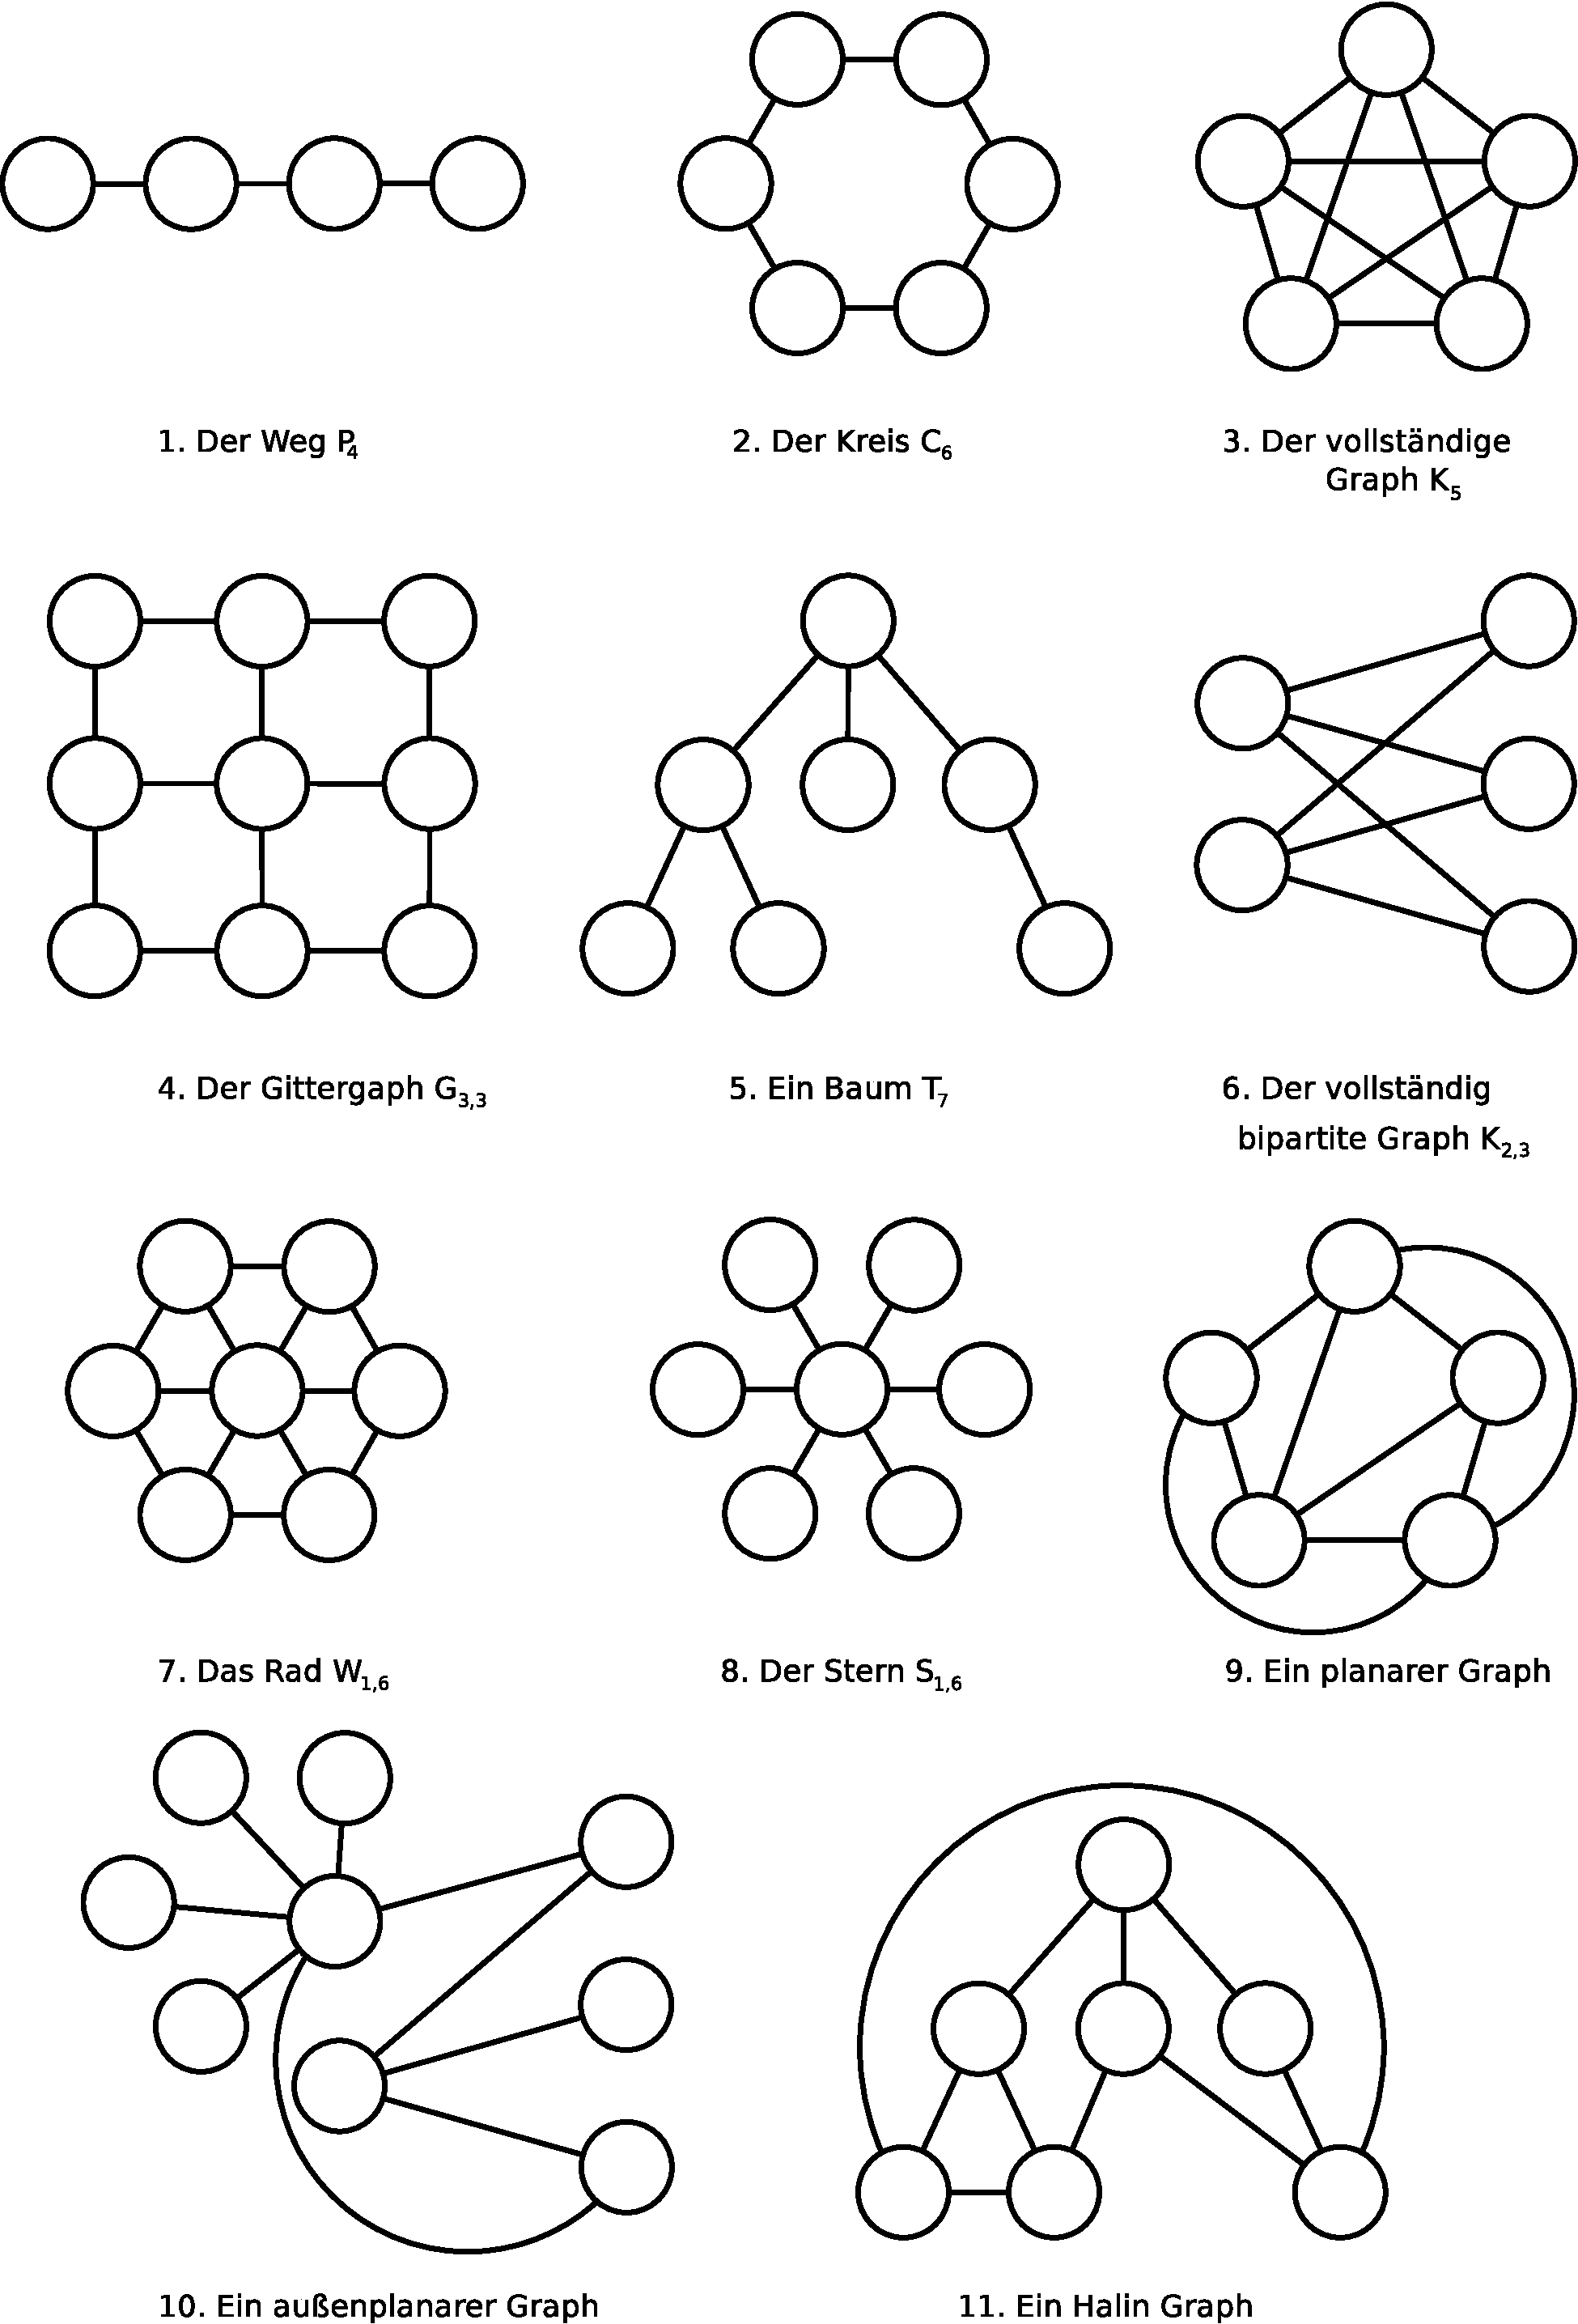
\includegraphics[width=430pt]{graphs.pdf}
	\caption{Beispiele einiger Graphklassen}
  	 \end{figure}
\clearpage
\subsection{Metrische Dimension}
\label{MDT}
\begin{defi}{\textbf{(Metrische Dimension)}}\\
\emph{Ein Knoten $x$ eines Graphen $G$ trennt zwei Knoten $u$ und $v$ in $G$ sofern $d(x, u) \neq d(x, v)$. Eine geordnete Knotenmenge $R$ von $G$ ist eine \emph{trennende Menge} von $G$ sofern je zwei unterschiedliche Knoten in $G$ durch mindestens einen Knoten in $R$ getrennt werden. Eine \emph{Metrische Basis} von $G$ ist eine trennende Menge mit minimaler Kardinalität, welche nicht eindeutig sein muss. Die Metrische Dimension $\beta(G)$ von $G$ ist die Kardinalität einer Basis\cite{?}. Gegeben seien eine endliche metrische Basis $R_n = \{r_1 , \ldots , x_n \} \subseteq V (G)$ und ein Knoten $t \in V (G)$, damit wird $(d(t, x_1 ), \ldots , d(t, x_n ))$ als der Vektor der \emph{Metrischen Koordinaten} von $t$ bezeichnet.} 
\end{defi}

\textbf{Bekannte Ergebnisse}\\
\begin{lem}
\label{path}
Die Metrische Dimension eines Graphens $G$ ist genau dann eins wenn der Graph $G$ ein Weg ist. (aus \cite{Landmarks})
\end{lem}
\begin{lem}
Die Metrische Dimension eines Baumes $T$, welcher keine Weg ist, lässt sich berechnen durch $\Sigma_{v \in V:L_v >1} (l_v-1)$.(Dabei ist $l_v$ die Anzahl der Brücken welche Wege sind am Knoten $v$ (aus \cite{Landmarks}))
\end{lem}
\begin{lem} 
Ein $d$-dimensionales Gitter $G_d$ hat $\beta(G_d)=d$ für $d \geq 2$.(aus \cite{Landmarks} und als falsch erklärt in \cite{some families of graphs})
\end{lem}
\begin{lem}
Ein Kreis $C_n$ der Ordnung $n$ hat $\beta(C_n)=2$.
\end{lem}
\begin{lem}
\label{stern}
Ein Stern $S_{1,n}$ hat $\beta(S_{1,n})=n-1$.
\end{lem}
\begin{lem}
Ein vollständiger Graph $K_n$ hat $\beta(K_n)=n-1$.
\end{lem}
\begin{lem}
\label{rad}
Ein Rad $W_{1,n}$ hat $\beta(W_{1,n})= \lfloor \dfrac{2n+2}{5} \rfloor$ für $n \notin \{3,6\}$ und $\beta(W_{1,n})=3$ für $n \in \{3,6\}$.
\end{lem}
\begin{lem}
Ein Graph $G$ mit $\beta(G) = k$ kann keinen $K_{2k+1}$ als Teilgraph beiinhalten. (aus \cite{Landmarks}))
\end{lem}
\begin{lem}
Sei $G = (V, E)$ ein Graph mit metrischen Dimension zwei, dann gilt folgendes: (aus \cite{Landmarks}))
\begin{enumerate}
\item Der $K_{5}$, sowie der $K_{3,3}$ sind keine Teilgraphen von $G$.
\item Ist $n \geq 3$ so kann der Graph $G$ ein Kreis $C_n$ sein.
\item Der Graph $W_{1,5}$ und $W_{1,6}$ haben metrische Dimension zwei.
\item Es gilt $\beta(P_m \square P_n)=2$. (2-dimensionales Gitter $n \times m$)
\end{enumerate}
\end{lem}

\begin{lem}
Sei $G = (V, E)$ ein Graph mit metrischer Dimension zwei und sei $\{a, b\} \subset V$ eine metrische Basis von $G$. Dann gilt folgendes:
\begin{enumerate}
\item Es existiert ein eindeutiger kürzester Weg $P$ zwischen $a$ und $b$.
\item Der Grad von $a$ und $b$ ist höchstens drei.
\item Jeder anderen Knoten auf dem Weg $P$ hat höchstens den Grad fünf.
\end{enumerate}
\end{lem}
\begin{lem}
Sei $G = (V, E)$ ein Graph mit $n$ Knoten und metrischer Dimension $n-2$, dann ist der Graph eines der folgenden: (aus \cite{Landmarks}))
\begin{enumerate}
\item Der $K_{r,s}$ mit $r,s \geq 1$.
\item Der $K_{r}+ \overline{K_s}$ mit $r,s \geq 1$.
\item oder der $K_{r,s}$ mit $r,s \geq 1$.
\end{enumerate}
\end{lem}
\begin{lem}
Sei ein außenplanarer Graph $G=(V,E)$ gegeben. Dann kann $\beta(G)$ in Polynomialzeit berechnet werden.(aus \cite{On the complexity})
\end{lem}
\todo[inline]{mehr bekannte resultate?} 
\textbf{NP-Vollständigkeitsresultate}
\begin{lem}
Sei ein beliebiger Graph $G=(V,E)$ gegeben. Das Minimurungsproblem für das Finden von $\beta(G)$ ist NP-vollständig.(aus \cite{On the complexity})
\end{lem}

\begin{lem}
Sei ein planarer Graph $G=(V,E)$ gegeben. Das Minimurungsproblem für das Finden von $\beta(G)$ ist NP-vollständig.(aus \cite{On the complexity})
\end{lem}

\begin{lem}
Sei ein bipartiter Graph $G=(V,E)$ gegeben. Das Minimurungsproblem für das Finden von $\beta(G)$ ist NP-vollständig.(aus \cite{An efficient representation of Benes networks and its applications})
\end{lem}

\textbf{Approximierbarkeit der metrischen Dimension}
\begin{lem}
Sei ein beliebiger Graph $G=(V,E)$ mit $n$ Knoten gegeben. Dann kann $\beta(G)$ approximiert werden mit dem Faktor von $O(log\:n)$ in Polynomialzeit.(aus \cite{Landmarks})
\end{lem}

\subsection{Metrische Dimension von zusammengestellten Graphen}
\begin{defi}{\textbf{(Vereinigung)}}\\
\emph{Gegeben seien zwei Graphen $G_1=(V_1,E_1)$ und $G_2=(V_2,E_2)$. Aus der Vereinigung $G_{1+2}=G_1+G_2$ entsteht der Graph mit der Knotenmenge $V_{1+2}=V_1 \cup V_2$ und der Kantenmenge $E_{1+2}= E_1 \cup E_2 \cup \{\{v_1,v_2\}| v_1 \in V_1 \wedge v_2 \in V_2\}$.} 
\end{defi}

\begin{defi}{\textbf{(Kartesisches Produkt)}}\\
\emph{Gegeben seien zwei Graphen $G_1=(V_1,E_1)$ und $G_2=(V_2,E_2)$. Aus dem kartesischen Produkt $G_{1\square 2}=G_1 \square G_2$ entsteht der Graph mit der Knotenmenge $V_{1 \square 2}=V_1 \times V_2$ und der Kantenmenge $E_{1\square 2}= \{\{(x_1,x_2),(y_1,y_2)\}| (x_1=y_1 \wedge \{x_2,y_2\} \in E_2)\vee (x_2=y_2 \wedge \{x_1,y_1\} \in E_1)\}$.} 
\end{defi}

\begin{defi}{\textbf{($r$-fache Verschmelzung)}}\\
\emph{Gegeben seien zwei Graphen $G_1=(V_1,E_1)$ und $G_2=(V_2,E_2)$ mit $|V_1|, |V_2| \geq r$ und zwei Teilmengen $V_{1,r} \subseteq V_1$ und $V_{2,r} \subseteq V_2$ mit $|V_{1,r}|, |V_{2,r}| = r$. Aus der $r$-fachen Verschmelzung $G_{1 \infty 2}=G_1 \infty G_2$ entsteht der Graph mit der Knotenmenge $V_{1 \infty 2}=V_1 \cup V_2\backslash V_{2,r}$ und der Kantenmenge $E_{1\infty 2}= E_1 \cup E_2$. Außerdem gilt, dass genau ein Knoten aus $V_{1,r}$ mit genau einem Knoten aus $V_{2,r}$ verschmolzen wird.} 
\end{defi}

\begin{defi}{\textbf{($r$-fache Vereinigung)}}\\
\emph{Gegeben seien zwei Graphen $G_1=(V_1,E_1)$ und $G_2=(V_2,E_2)$ mit $|V_1|, |V_2| \geq r$ und zwei Teilmengen $V_{1,r} \subseteq V_1$ und $V_{2,r} \subseteq V_2$ mit $|V_{1,r}|, |V_{2,r}| = r$. 
Aus der $r$-fachen Vereinigung $G_{1 \leftrightarrow 2}= G_1 \leftrightarrow G_2$ entsteht der Graph mit der Knotenmenge $V_{1 \leftrightarrow 2}=V_1 \cup V_2$ und der Kantenmenge $E_{1\leftrightarrow 2}= E_1 \cup E_2 \cup E_{\leftrightarrow }$ mit $E_{\leftrightarrow}=\{\{v_1,v_2\}| v_1 \in V_{1,r} \wedge v_2 \in V_{2,r} \}$ und dabei gilt für jedes $v_1 \in V_{1,r}$ das $|\{\{v_1,v_2\} \in E_{\leftrightarrow} \wedge  v_2 \in V_{2,r} \}|= 1$ und für jedes $v_2 \in V_{2,r}$ das $|\{\{v_1,v_2\} \in E_{\leftrightarrow} \wedge v_1 \in V_{1,r} \}|= 1$ .} 
\end{defi}

\begin{lem}(Bekannte Ergebnisse für Vereinigung und für das kartesische Produkt)
\begin{itemize}
\item $max\{\beta(G),\beta(H)\}\leq \beta(G\square H) \leq min\{\beta(G)+|H|,\beta(H)+|G|\}-1$
\item $2 \leq \beta(G) \leq \beta(H) \leq \beta(G\square H) \leq min\{\beta(G)+|H|,\beta(H)+|G|\}-2$
\item $\beta(G)+\beta(H) \leq \beta(G+H)$
\end{itemize} 
(aus \cite{some families of graphs})
\end{lem}

\begin{lem}(Bekannte Ergebnisse für das kartesische Produkt spezieller Graphen)
\begin{itemize}
\item $\beta(G)\leq \beta(G\square K_2) \leq \beta(G)+1$
\item $\beta(G)\leq \beta(G\square P_n) \leq \beta(G)+1$
\item $\beta(G\square K_n) \leq \beta(G)+n-2$ für $n \geq 3$
\item $\beta(G\square C_n) \leq \beta(G)+1$ für $n$ ungerade
\item $\beta(G\square C_n) \leq \beta(G)+2$ für $n$ gerade
\item $\beta(P_m+P_n)=2$
\item $\beta(P_m+K_n)=n-1$ für $n\geq 3$
\item $\beta(P_m+C_n)=2$ für $n$ ungerade
\item $\beta(P_m+C_n)=2$ für $n$ gerade und $m \neq 1$
\item $\beta(C_m+C_n)=3$ falls $m$ oder $n$ gerade
\item $\beta(C_m+C_n)=4$ sonst
\item $\beta(K_m+C_n)=m$ falls $m=4$ und $n$ ungerade
\item $\beta(K_m+C_n)=m-1$ sonst
\end{itemize} 
(aus \cite{some families of graphs})
\end{lem}

\begin{lem}$\;\;$\\Folgende Schranken gelten für die $r$-fache Verschmelzung von Graphen mit $r \geq 4$:
$$\beta(G_1)+\beta(G_2)-2r \leq \beta(G_1 \infty G_2) \leq \beta(G_1)+\beta(G_2)+r+\lceil\frac{r-4}{2}\rceil$$
\end{lem}

\begin{proof}[Beweis:] 
Um zu zeigen dass die Schranken strikt sind werden zwei folgende Klassen von Graphen betrachtet.\\
Für die untere Schranke gilt:
\end{proof}
\section{Metrische Dimension zweier Graph Klassen}
\subsection{Stuktur Eigenschaften}
\begin{lem}
Die metrische Dimension eines Teilgraphen ist nicht durch die metrische Dimension des ursprünglichen Graphen beschränkt. (Durch das Entfernen von Kanten kann die metrische Dimension eines Graphen steigen.)
\end{lem}
\begin{proof}[Beweis:]$\;$\\
Das Rad $W_{1,6}$ hat nach Lemma \ref{rad} metrische Dimension $3$. Durch das Entfernen von allen Kanten auf dem äußeren Kreis entsteht der Stern $S_{1,6}$ mit der metrischen Dimension $5$ nach Lemma \ref{stern}.
\end{proof}
Durch das Löschen von Kanten kann eine Verringerung der metrischen Dimension um $$n-1-\lfloor \dfrac{2n+2}{5} \rfloor=_{da \:n-1 \in \mathbb{N}}\lfloor n-1- \dfrac{2n+2}{5} \rfloor=\lfloor \dfrac{3n-7}{5} \rfloor$$ für $n \in {4,5}$ und $n > 6$ erreicht werden.
\begin{lem}
Die metrische Dimension eines induzierten Teilgraphen ist nicht durch die metrische Dimension des ursprünglichen Graphen beschränkt. (Durch das Entfernen von Knoten kann die metrische Dimension eines Graphen steigen.)
\end{lem}
\begin{proof}[Beweis:]$\;$\\

\begin{figure}[h!]
		\centering 		 
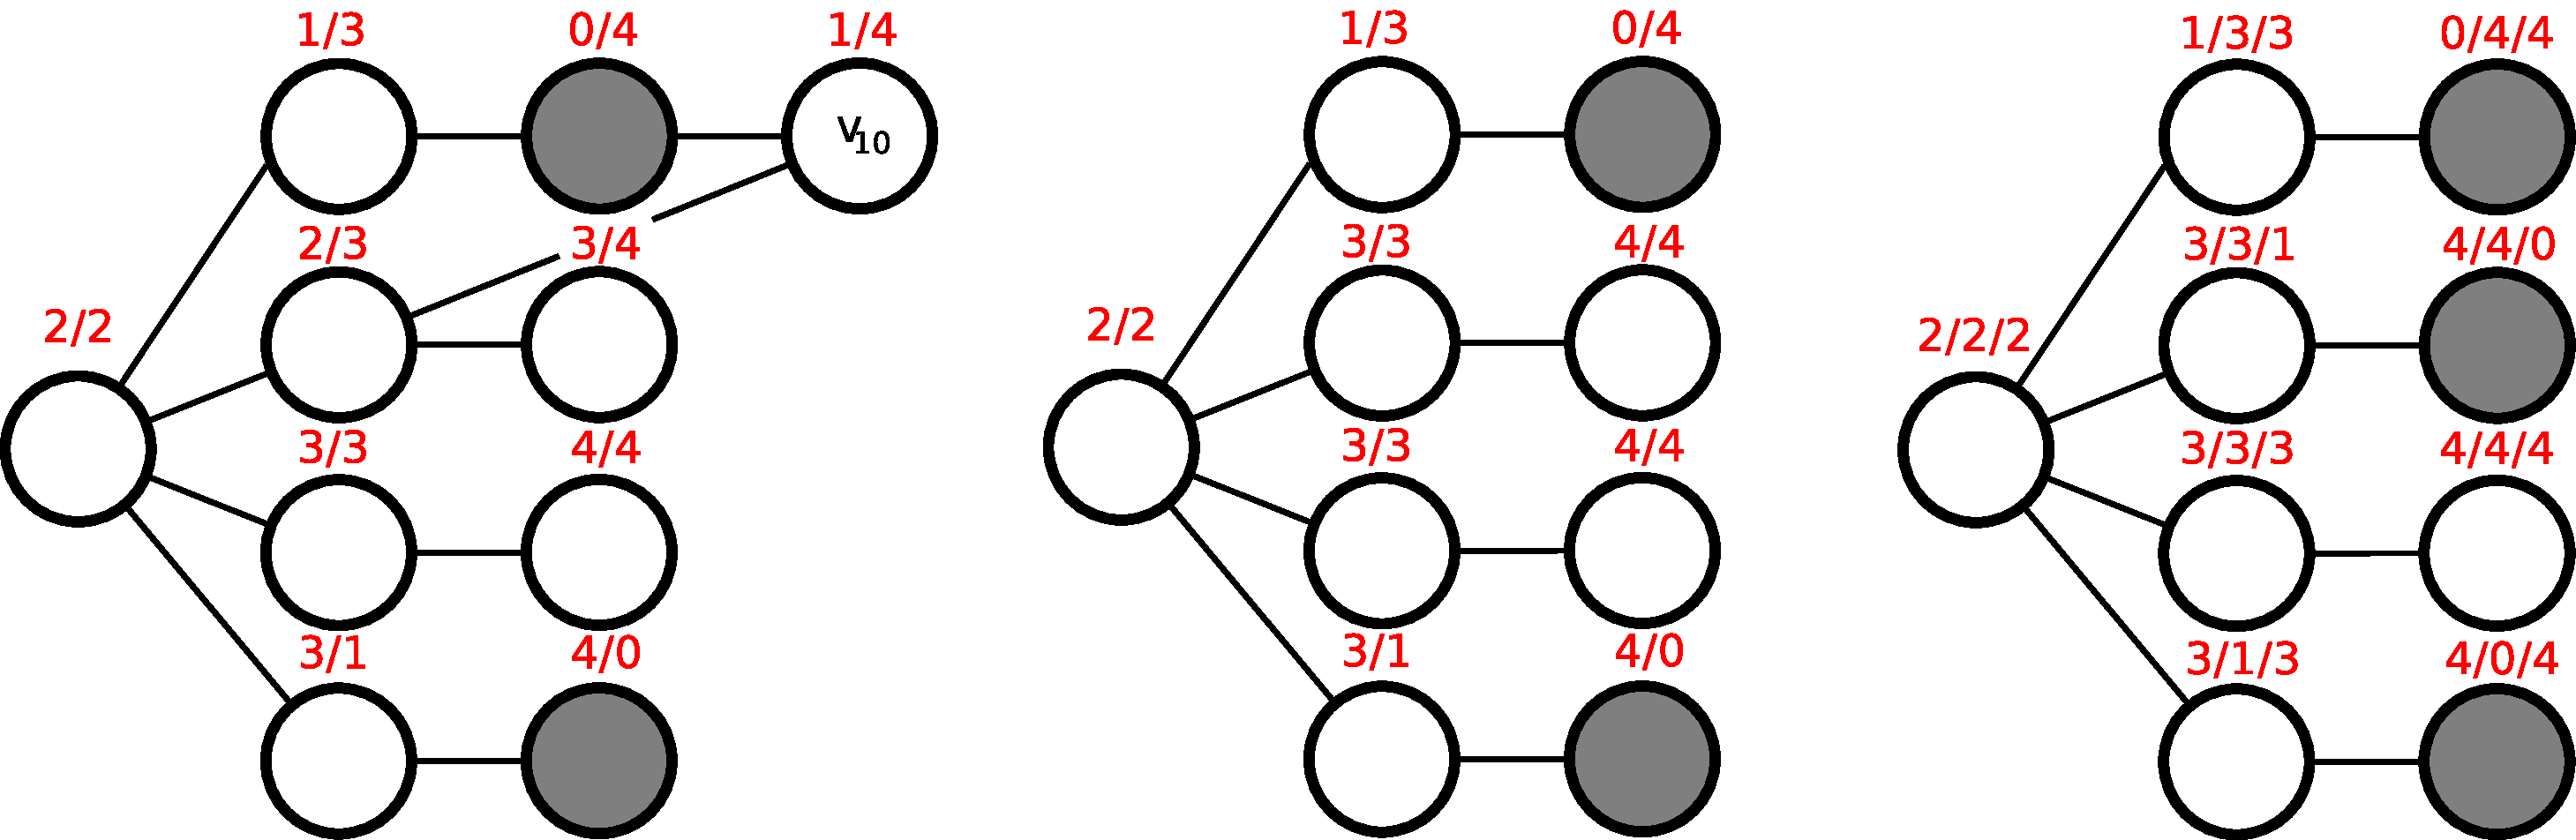
\includegraphics[width=420pt]{example.pdf}
   \caption{Beispiel für einen Teilgraphen mit größerer MD als der Graph selbst}
  	 \end{figure}
  	 Betrachtet werden die folgenden zwei Graphen $G_{10}$ und $S_{1,4,2}$.
Obwohl der $G_{10}$ durch das Entfernen von $v_{10}$ zum $S_{1,4,2}$ wird und somit der $S_{1,4,2}$ ein induzierter Teilgraph vom $G_{10}$ ist, gilt dass $\beta(G_{10})=2$ und $\beta(S_{1,4,2})=3$.
\end{proof}
\begin{lem}
\label{dist}
Sei $G=(V,E)$ ein gegebener Graph. Seien $u,v$ und $w$ Knoten in $G$ und sei $\{u,v\}\in E$. Sei $d$ die Länge eines kürzesten Weges von $u$ zu $w$ in $G$. Dann ist die Länge eines kürzesten Weges von $v$ zu $w$ ein Element der Menge $\{d-1,d,d+1\}$. (aus \cite{Landmarks})
\end{lem}
\begin{lem}
\label{trennungsknoten}
Sei ein beliebiger Graph $G=(V,E)$ gegeben. Seien $G_1$ und $G_2$ zwei disjunkte Teilgraphen von $G$ die durch das Löschen von einem Knoten $x$ entstehen. Die Menge der getrennten Knoten in $G_2$ von Elementen aus der metrischen Basis aus $G_1$ ist übereinstimmend mit der Menge der getrennten Knoten in $G_2$ sofern nur $x$ in der metrischen Basis wäre. Und umgekehrt gilt dasselbe für die Knoten in $G_1$.
\end{lem}
\begin{lem}
\label{sepvertex}
Sei ein beliebiger Graph $G=(V,E)$ mit der metrischen Dimension $r$ gegeben. Sei $G*$ ein Teilgraph von $G$ mit der metrischen Dimension $k \leq r$ und der metrischen Basis $R_k$. Die Anzahl der Trennungsknoten vom Grad zwei summiert mit der Anzahl der Elemente aus der metrischen Basis von $G*$ hat mindestens die Größe der metrischen Dimension vom Teilgraphen. Der Knoten, welcher mit dem Trennungsknoten verbunden ist wird als $v_t$ bezeichnet.
\end{lem}
\begin{proof}[Beweis mittels vollständiger Induktion über die Anzahl der Trennungsknoten:]$\;$
\begin{itemize}
\item[IA:] Sei der Graph $G*$ nur über einen Knoten vom Grad zwei mit dem Restgraphen verbunden. Werden dieselben Elemente in die metrische Basis aufgenommen wie zuvor, so werden alle Knoten in $G*$ getrennt. 
Wird ein Element aus $G\setminus{G*}$ in die metrische Basis aufgenommen, so kann höchstens ein Element aus $R_k$ entfernt werden. 
\item[IV:] 
\item[IS:]
\end{itemize}
\end{proof}
\begin{lem}
\label{first_theorem}
Gegeben ein Graph bestehend aus zwei Teilgraphen $G_R$ und $G_L$, welche durch genau eine Kante verbunden sind. Sofern jeder Teilgraph mind. ein Element aus der metrischen Basis beinhalten, so ist jedes Knotenpaar $x,y$ mit der Eigenschaft $x \in G_R$ und $y \in G_L$ getrennt.
\end{lem}

\begin{proof}[Beweis:]
\textcolor{white}{x}
\begin{figure}[h!]
		\centering 		 
  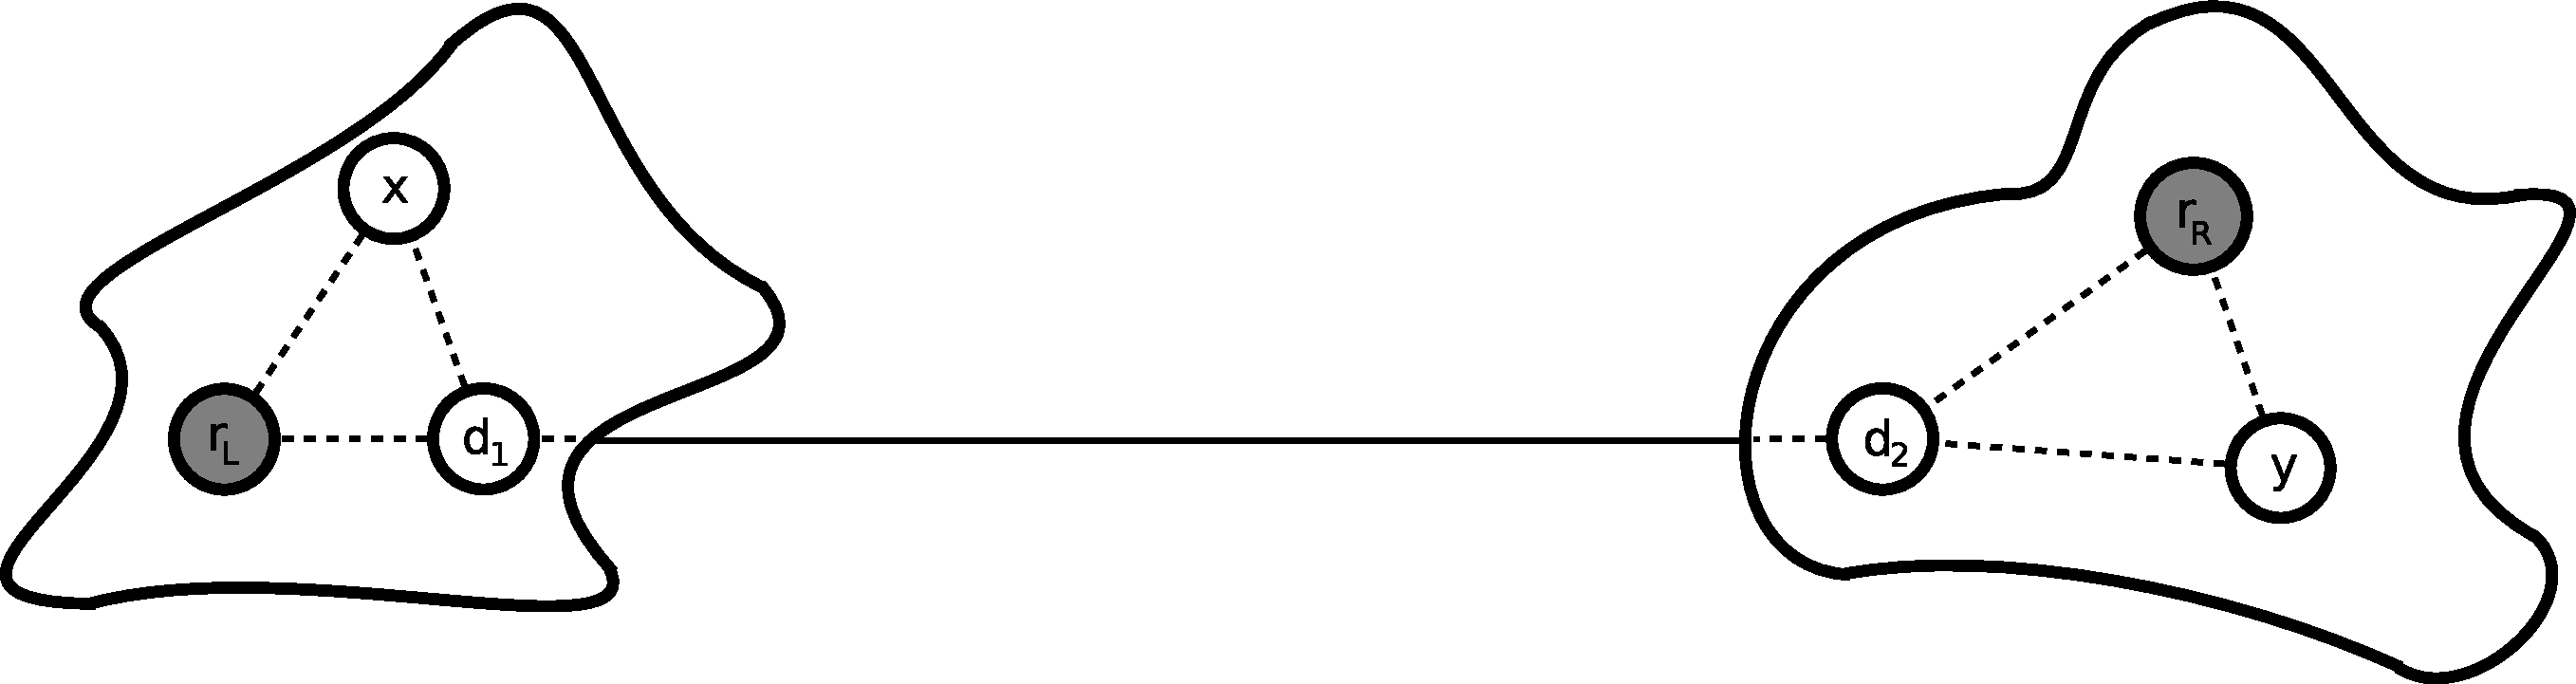
\includegraphics[width=420pt]{bew5.pdf}
	\caption{Ein Graph mit zwei über eine Kante verbundenen Teilgraphen mit jeweils einem Element aus der metrischen Basis}
  	 \end{figure}
  Angenommen es existiert ein nicht getrenntes Knotenpaar $x,y$. Sei $d_1$ der Bifurkator von $y,x,r_L$ und $d_2$ der Bifurkator von $x,y,r_R$. Dann gilt: $$dist(r_L,x) \leq dist(r_L,d_1)+ dist(d_1,x)$$ $$dist(r_R,y) \leq dist(r_R,d_2)+ dist(d_2,y)$$ $$dist(r_L,y) > dist(r_L,d_1)+ dist(d_2,y)$$ $$dist(r_R,x) > dist(r_R,d_2)+ dist(d_1,x)$$
  Da $x$ und $y$ nicht getrennt sind, gilt:
   $$dist(r_R,y) =dist(r_R,x),\: dist(r_L,x) = dist(r_L,y)$$ Dies kann eingesetzt und umgeformt werden zu dem folgenden Widerspruch:
  $$\Rightarrow dist(r_L,d_1)+ dist(d_1,x) \geq dist(r_L,x) = dist(r_L,y)> dist(r_L,d_1)+ dist(d_2,y)$$
  $$\Leftrightarrow dist(r_L,d_1)+ dist(d_1,x) > dist(r_L,d_1)+ dist(d_2,y)$$
  $$\Leftrightarrow dist(d_1,x) >  dist(d_2,y)$$
  
  $$\Rightarrow dist(r_R,y) \leq dist(r_R,d_2)+ dist(d_2,y) < dist(r_R,d_2) + dist(d_1,x) < dist(r_R,x)$$
  $$\Leftrightarrow dist(r_R,y) < dist(r_R,x) = dist(r_R,y)$$
  $$\Leftrightarrow dist(r_R,y) < dist(r_R,y) \lightning $$  
  
\end{proof}
\begin{lem}
\label{lem2}
Die Kontraktion von Trennungsknoten vom Grad zwei oder die Knotenerweiterung hat keinen Einfluß auf die metrische Dimension eines Graphens.
\end{lem}
\begin{proof}[Beweis:]
Sei ein Graph $G$ mit einer metrischen Basis $R_k$ und einem Trennungsknoten $v_s$ mit $deg(v_s)=2$ gegeben. Die zwei Teilgraphen welche durch das Entfernen von $v_s$ entstehen bezeichne man als $G_R$ und $G_L$. Der Graph $G'$ resultiert durch die Kontraktion von $v_s$ mit einem beliebigen Nachbarn.\\
Angenommen die metrische Dimension in $G'$ ist größer als in $G$, dann existiert ein Knotenpaar $x,y$, welcher in $G$ getrennt wird, aber nicht in $G'$. Also gibt es mindestens einen Knoten in der metrischen Basis $R_K$ von dem Graphen $G$, welcher $x,y$ trennt. Sei dies der Knoten $r_k$. Dieser Knoten trennt  $x,y$ nicht in dem Graphen $G'$.\\
Betrachte nun die Fälle einzeln: Falls alle drei Knoten in dem gleichen Teilgraphen sind, so ist $v_s$ in keinem kürzesten Weg enthalten und $x,y$ bleiben getrennt, sofern sie zuvor getrennt waren. Sind die Knoten $x,y$ in einem Teilgraphen und $r_k$ in dem Anderen, so schrumpft die kürzeste Wege Distanz von $r_k$ zu $x$ und zu $y$ um genau eins und bleibt dabei unterschiedlich auch in $G'$. Betrachte nun den Fall dass die Knoten $x$ und $y$ in unterschiedlichen Teilgraphen sind:
  \begin{figure}[h!]
		\centering 		 
  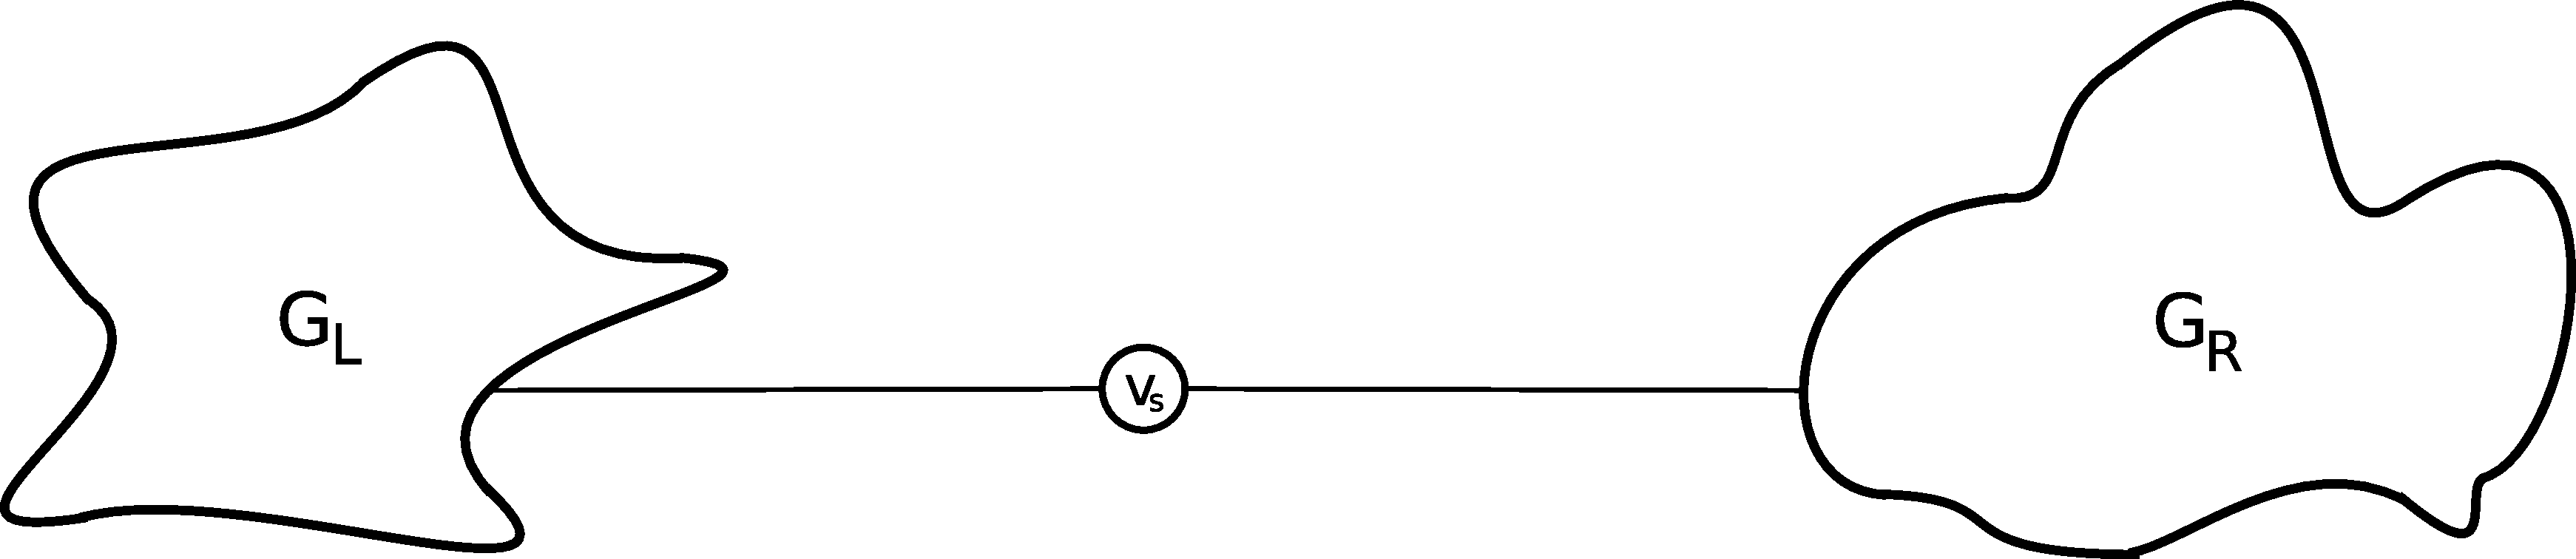
\includegraphics[width=425pt]{proof4.pdf}
	\caption{Ein Graph mit einem Trennungknoten vom Grad zwei}
  	 \end{figure}
\begin{enumerate}
\item[1. Fall] Angenommen jeder der Teilgraphen $G_R$ und $G_L$ beinhalten mind. ein Element aus der metrischen Basis. Der Widerspruch folgt unmittelbar aus dem Satz \ref{first_theorem}.
\item[2. Fall] Angenommen einer der Tielgraphen beinhaltet kein Element der metrischen Basis, sei dies o.B.d.A $G_R$.
Dadurch das dieser Teilgraph kein Element der metrischen Basis beinhaltet und genau einen Trennungsknoten besitzt folgt aus dem Satz \ref{sepvertex} das die metrische Dimension von $G_R$ höchstens eins ist und da $G_R$ nicht leer ist gilt nach Satz \ref{path} dass $G_R$ ein Weg ist. Falls ein nichtgetrenntes Paar von Knoten $x,y$ existiert mit o.B.d.A. $x$ ist im Teilgraphen $G_R$, dann war in $G$ das Knotenpaar $x$ und der Vorgänger von $y$ nicht getrennt. Damit ist auch der letzte Widerspruch gezeigt.
%\item[3.b. Case]  O.B.d.A. sei $G_R$ der Teilgraph, der ein Weg ist. Damit besteht das Resolving Set $R_K$ aus mind. 2 Knoten. Ist einer davon im $G_R$, dann gilt das gleiche Argument wie im Fall 3(a) und das Knotenpaar $x,y$ ist getrennt.\\Sind alle Knoten aus dem Resolving Set im $G_L$ und ist die Entfernung von allen Knoten zu $x$ und $y$ gleich im $G'$, so war die Entfernung zu $x$ und zu dem Vorgänger von $y$ gleich, und damit wäre $R_k$ ursprünglich kein gültiges Resolving Set in $G$ gewesen.

\end{enumerate}
Für den Fall dass die metrische Dimension in $G'$ kleiner ist als in $G$ wird der Beweis analog geführt.
%\textbf{Angenommen $MD(G')<MD(G)$:}\newline\newline Dann gibt es mind. einen überflüssigen Knoten im $R_K$ mit der Bezeichnung $r_{k'}$. . Seien diese aus dem Resolving Set $R'_K$ entfernt worden. Seien $x,y$ zwei Knoten die im $G$ bzgl. $R'_K$ gleiche Markierungen hatten, und im $G'$ nicht.\\
%Liege $r_{k'}$ im gleichen Teilgraphen wie $x,y$, so kann der Knoten $v_s$ auf keinem kürzesten Weg gewesen sein und so wäre $R_K$ in $G$ ein Resolving Set gewesen.\\
%Sind $x,y$ in einem anderen Teilgraphen als $r_{k'}$, so liegt $v_s$ auf beiden kürzesten Wegen und so verringern sich beide Markierungen um genau eins. Damit bleiben sie getrennt oder $R_K$ in $G$ ist ein Resolving Set.\\
%Sei nun einer der ursprünglich nichtgetrennten Knoten und der trennende Knoten $r_{k+1}$ in dem gleichen Teilgraphen. Sei dies o.B.d.A. $x$.\\
%\textbf{Fall (i):} $G_R$ und $G_L$ sind Wege. Dann gibt es genau einen Knoten im Resolving Set und die Knoten sind getrennt sofern sie zuvor getrennt waren, da die Anzahl der Knoten auf einem Weg irrelevant ist.\\
%\textbf{Fall (ii):} O.B.d.A. sei $G_R$ der Teilgraph, der ein Weg ist. Damit besteht das Resolving Set $r$ aus mind. 2 Knoten. Ist einer davon im $G_R$, dann gilt gleiches Argument wie in Fall (i) und das Knotenpaar $x,y$ ist getrennt.\\Sind alle Knoten aus dem Resolving Set im $G_L$ und ist die Entfernung von allen Knoten zu $x$ und $y$ gleich im $G'$, so war die Entfernung zu $x$ und zu dem Vorgänger von $y$ gleich, und damit wäre $R_k$ ursprünglich kein gültiges Resolving Set.\\
%\textbf{Fall (iii):} $G_R$ und $G_L$ sind keine Wege. Damit ist in jedem Teilgraphen mind. ein Element aus dem Resolving Set. Und die Widerspruch folgt aus nach Satz 1.1.\newline\newline
\end{proof}
\subsection{Metrische Dimension von $C_j$-Bäumen}
In diesem Kapitel wird eine neue Graphklasse eingeführt. Es sind Bäume mit der Eigenschaft, dass Knoten mit größerem Grad als zwei durch Kreise ersetzt werden. Das Kapitel widmet sich der Bestimmung der metrischen Dimension solcher Graphen sowie dem Vergleich der metrischen Dimension von den ursprünglichen Bäumen gegenüber den mit den Kreisen erweiterten. 
\begin{defi}
\label{C_{3,j} tree}
\textcolor{white}{x}
Für einen gegebenen Baum $T=(V,E)$ mit $deg(v_i)\leq 3$ für $v_i \in V$, wird der $C_{3,j}$-Baum folgend gebildet:
   Sei $$V'=\{v_k|v_k \in V \wedge deg(v_k)=3\}\subseteq V$$ eine Teilmenge der Knoten von dem Graphen $T$. Ersetze jedes Element $v_j \in V'$ durch einen $C_3$ (diese Teilgraphen werden als \emph{$C_{3,j}$} bezeichnet), so dass jeder Knoten vom $C_{3,j}$ mit genau einem Nachbarn von $v_j$ verbunden wird. Die drei Nachbarn vom $C_{3,j}$ werden als \emph{$C_{3,j}$-$Kinder$} bezeichnet. Sofern zwei von den $C_{3,j}$-$Kinder$ Blätter sind, so bezeichnet man den Teilgraphen mit dem $C_{3,j}$ und seinen Nachbarn als \emph{$C_{3,j}$-$Blatt$}.
   \end{defi}
\todo{Aufbau: Baum und Kreise mit Grad 3}
\begin{bsp}

\clearpage
\begin{figure}[h!]
		\centering 		 
   \includegraphics[width=430pt]{trees3.pdf}
	\caption{Entwicklung von einem Baum zum $C_{3,j}$-$Baum$ und anschließender Knotenkontraktion}
  	 \end{figure}
\end{bsp}
Die metrische Dimension (MD) eines Graphen $G$ mit mindestens zwei $C_{3,j}$ ist gleich der Anzahl von seiner $C_{3,j}$-$Blätter$.
\begin{lem}
Sei $C_{3,j}$ ein beliebiges $C_{3,j}$-$Blatt$. Jede metrische Basis muss mindestens eine der folgenden Knoten $\{v_{j,1},v_{j,2},v_{j,3},v_{j,4}\}$ beinhalten.
\end{lem}
\begin{proof}[Beweis:]
Angenommen keiner dieser Knoten ist in der metrischen Basis. Durch die eindeutige Verbindung zu dem Restgraphen, welche über einen Trennungsknoten läuft, folgt aus Symmetriegründen dass die Knoten $v_{j,3}$ und $v_{j,4}$, sowie $v_{j,1}$ und $v_{j,2}$ identische Markierungen haben. Dies ist ein Widerspruch zu der Definition einer metrischen Basis.

\clearpage
\begin{figure}[h!]
		\centering 		 
	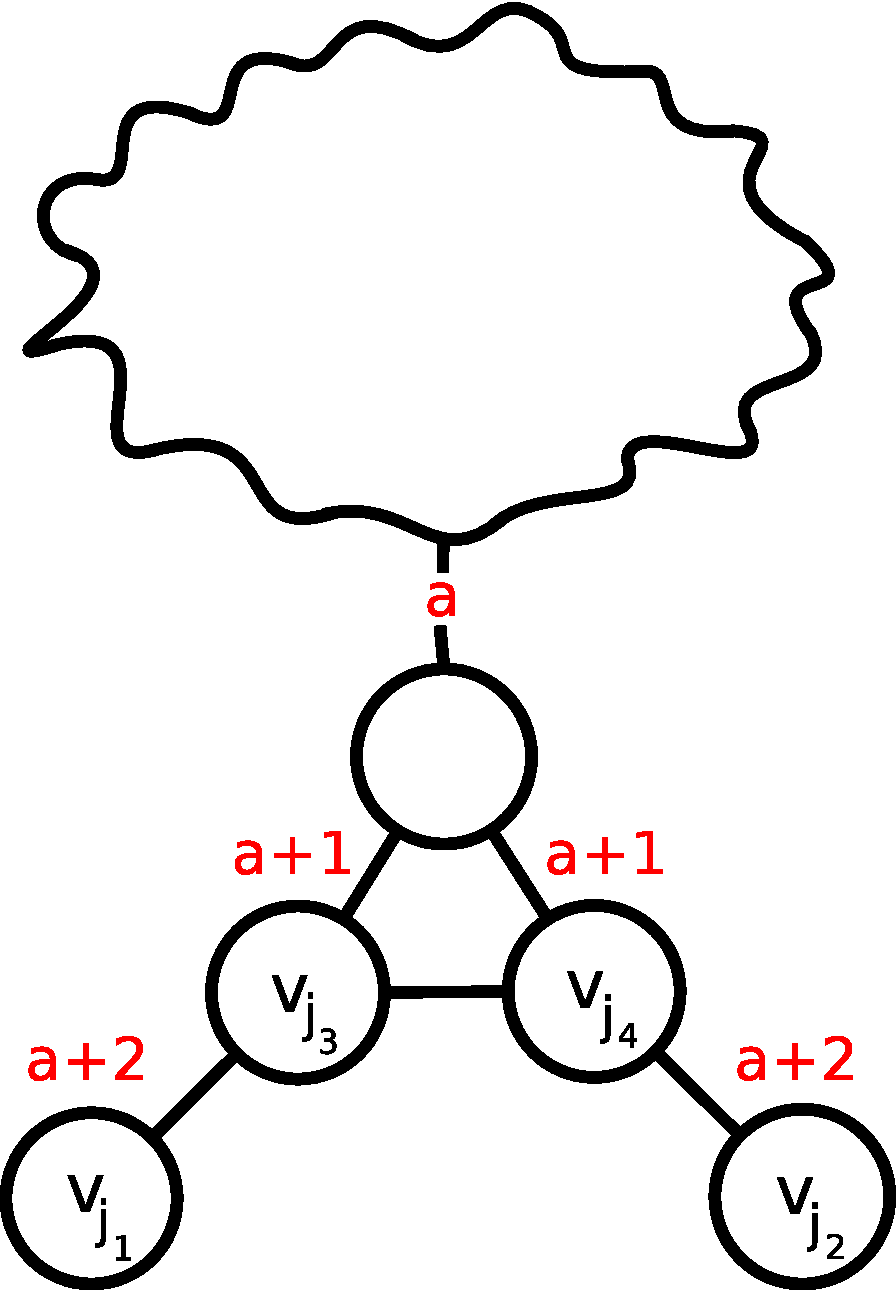
\includegraphics[width=150pt]{beweis.pdf}
	\caption{Die Markierungen eines $C_{3,j}$-$Blattes$ ohne das ein Knoten von diesem in der metrischen Basis ist}
  	 \end{figure}
Damit ist die metrische Dimension eines Graphens $G$ mit mindestens zwei $C_{3,j}$ mindestens gleich der Anzahl von seinen $C_{3,j}$-$Blättern$.
\end{proof}
\begin{lem}
Die metrische Dimension (MD) eines Graphen $G$ mit mindestens zwei $C_{3,j}$ ist nicht größer als die Anzahl seiner $C_{3,j}$-$Blätter$. 
\end{lem}
Um diese Eigenschaft zu beweisen werden zwei Sätze über die Struktur solcher $C_{3,j}$-$Bäume$ benötigt.
\begin{lem}
Jeder Knoten eines $C_{3,j}$-$Baumes$, welcher kein Blatt ist, ist ein Trennungsknoten.
\end{lem}
\begin{proof}[Beweis:]
Angenommen es gibt einen Knoten $u$, welcher kein Blatt ist und kein Trenunngsknoten. Da der Graph nur aus Knoten von Grad drei und Grad eins besteht ist der Knotengrad von $u$ drei. Dies bedeutet $u$ hat genau drei Nachbaren $v,w,x$. Da
der Knoten $u$ ist nach Annahme kein Trennungsknoten und somit gibt es einen Weg zwischen jedem Paar seiner Nachbarknoten.\begin{itemize}
\item Fall I: Ein Nachbarknoten ist ein Blatt.\\ Es kommt direkt zum Widerspruch, da durch das Löschen von $u$ sich der Knotengrad von dem Blatt um eins verkleinert und damit null wird, also ein getrennter einzelner Knoten ist.\item
Fall II: Alle Nachbarknoten haben den Grad drei.\\
Es muss immernoch einen Weg zwischen jedem Knotenpaar geben damit der Graph zusammenhängend ist. Somit gibt es auch einen kürzesten Weg über alle drei Knoten, sei der Anfangsknoten von diesem Weg o.B.d.A. der Knoten $v$, der Endknoten o.B.d.A. der Knoten $x$ und die Länge dieses Weges ist zwangsläufig mindestens drei. Wird wieder der entfernte Knoten $u$ betrachtet so folgt, dass der Graph einen Kreis beinhaltet welcher aus dem Weg von $v$ zu $x$ besteht und über den entfernten Knoten $u$ zurück zum Knoten $v$.\\
Damit gibt es in dem Graphen mind. einen Kreis mit einer echt größeren Länge als drei und dies ist ein Widerspruch zur Definition des $C_{3,j}$-$Baumes$, welche nur Kreise der Länge drei erlaubt.
\end{itemize}
\end{proof}
\begin{lem}
In jedem Teilgraphen eines $C_{3,j}$-$Baumes$ mit mindestens vier Knoten ist mindestens ein Knoten aus der metrischen Basis.
\end{lem}
\begin{proof}[Beweis:]
Der kleinste Teilgraph der durch das Löschen eines Knotens entstehen kann ist ein Blatt. Dieser besteht allerdings nur aus einem Knoten. Der nächstgrößere Teilgraph der durch das Löschen eines Knotens entstehen kann beinhaltet vier Knoten und zwar den unteren Teil eines $C_{3,j}$-$Blattes$. Somit beinhaltet er auch sein linkes Blatt, welches in die metrische Basis aufgenommen wird. Jeder größere Teilgraph beinhaltet diese vier Knoten. %Unabhängig davon welcher Knoten als Wurzel verwendet wurde, galt bei dem ursprünglichen Baum dass der Knoten mit der weitesten Entfernung von der Wurzel(der Knoten davor), hatte genau zwei Kinder und aus dem wurde ein $C_{3,j}$-$Blatt$.  
\end{proof}
\begin{proof}[Beweis von Lemma 27:]
Der gesamte Graph besteht nur aus Knoten vom Grad drei oder Grad eins. In die metrische Basis wird das linke Blatt von jedem $C_{3,j}$-$Blatt$ aufgenommen. Sei $n$ die Anzahl der $C_{3,j}$-$Blätter$ und $m$ die Anzahl der $C_{3,j}$, die keine $C_{3,j}$-$Blätter$ sind und bei diesem Beweis als einfache $C_{3,j}$ bezeichnet werden.\\
\begin{itemize}
\item Fall I. Die Knoten $u$ und $v$ haben unterschiedliche Distanzen vom Knoten $r$ aus der metrischen Basis:\\
Der Knoten $r$ trennt die Knoten $u$ und $v$.
\item Fall II. Die Knoten $u$ und $v$ haben die gleiche Distanz vom Knoten $r$ aus der metrischen Basis und die Knoten $u$ und $v$ liegen im selben $C_{3,j}$.\\
O.B.d.A. sei $b_1$ der ausgewählte Knoten $r$ oder $b_1$ auf allen kürzesten Wegen von dem Knoten $r$ zu jedem Knoten in dem $C_{3,j}$. Es gibt zwei nicht getrennte Knotenpaare durch den Knoten $r$ entweder das Knotenpaar $b_2$ und $b_3$, oder das Knotenpaar $c_2$ und $c_3$.\\
Angenommen $b_2$ und $b_3$ sind Blätter (daraus folgt das $b_1$ kein Blatt sein kann), so wird o.B.d.A. $b_3$ in die metrische Basis aufgenommen und so ist seine Markierung o.B.d.A. an der ersten Position $0$ und er ist der einzige Knoten mit dieser Markierung. Sein einziger Nachbar $c_3$, bekommt die Markierung $1$ an der ersten Position, damit ist dieser Knoten auch eindeutig markiert. Die anderen zwei Knoten $c_1$ und $c_2$ auf dem $C_3$ bekommen die Markierung $2$ an der ersten Position und ihre zwei Nachbaren $b_1$ und $b_2$, die Markierung $3$ an der ersten Position. Somit kriegen die Knotenpaare $b_2$ und $b_3$ und $c_2$ und $c_3$ unterschiedliche Markierungen und sind getrennt.\\
Sei nun $b_3$ kein Blatt, damit ist er Teil eines anderen $C_{3,j}$, welcher zwei $C_{3,j}$-$Kinder$ besitzt, sind beide keine Blätter, so sind sie Teile eines anderen $C_{3,j}$. Da der betrachtete Graph aber nach Vorraussetzung endlich ist und keine größeren Kreise besitzt als den $C_3$, stößt man auf ein $C_{3,j}$-$Blatt$, wessen linkes Blatt in die metrische Basis aufgenommen wurde. Die Distanz von diesem Knoten zu $b_3$ ist echt kleiner als zu jedem anderen Knoten in dem ausgewählten $C_{3,j}$, da der Knoten $b_3$ auf dem einzigen Weg zu den anderen Knoten auf dem $C_{3,j}$ liegt. Diese Aussage gilt aufgrund der ursprünglichen Baumstruktur des Graphen. Die Markierung von $b_3$ sei o.B.d.A. an der ersten Position $x$. Sein einziger Nachbar $c_3$, bekommt die Markierung $x+1$ an der ersten Position. Die anderen zwei Knoten $c_1$ und $c_2$ auf dem $C_3$ bekommen die Markierung $x+2$ an der ersten Position und ihre zwei Nachbaren $b_1$ und $b_2$, die Markierung $x+3$ an der ersten Position. Somit kriegen die Knotenpaare $b_2$ und $b_3$ und $c_2$ und $c_3$ unterschiedliche Markierungen und sind getrennt.

\begin{figure}[h!]
		\centering
 		 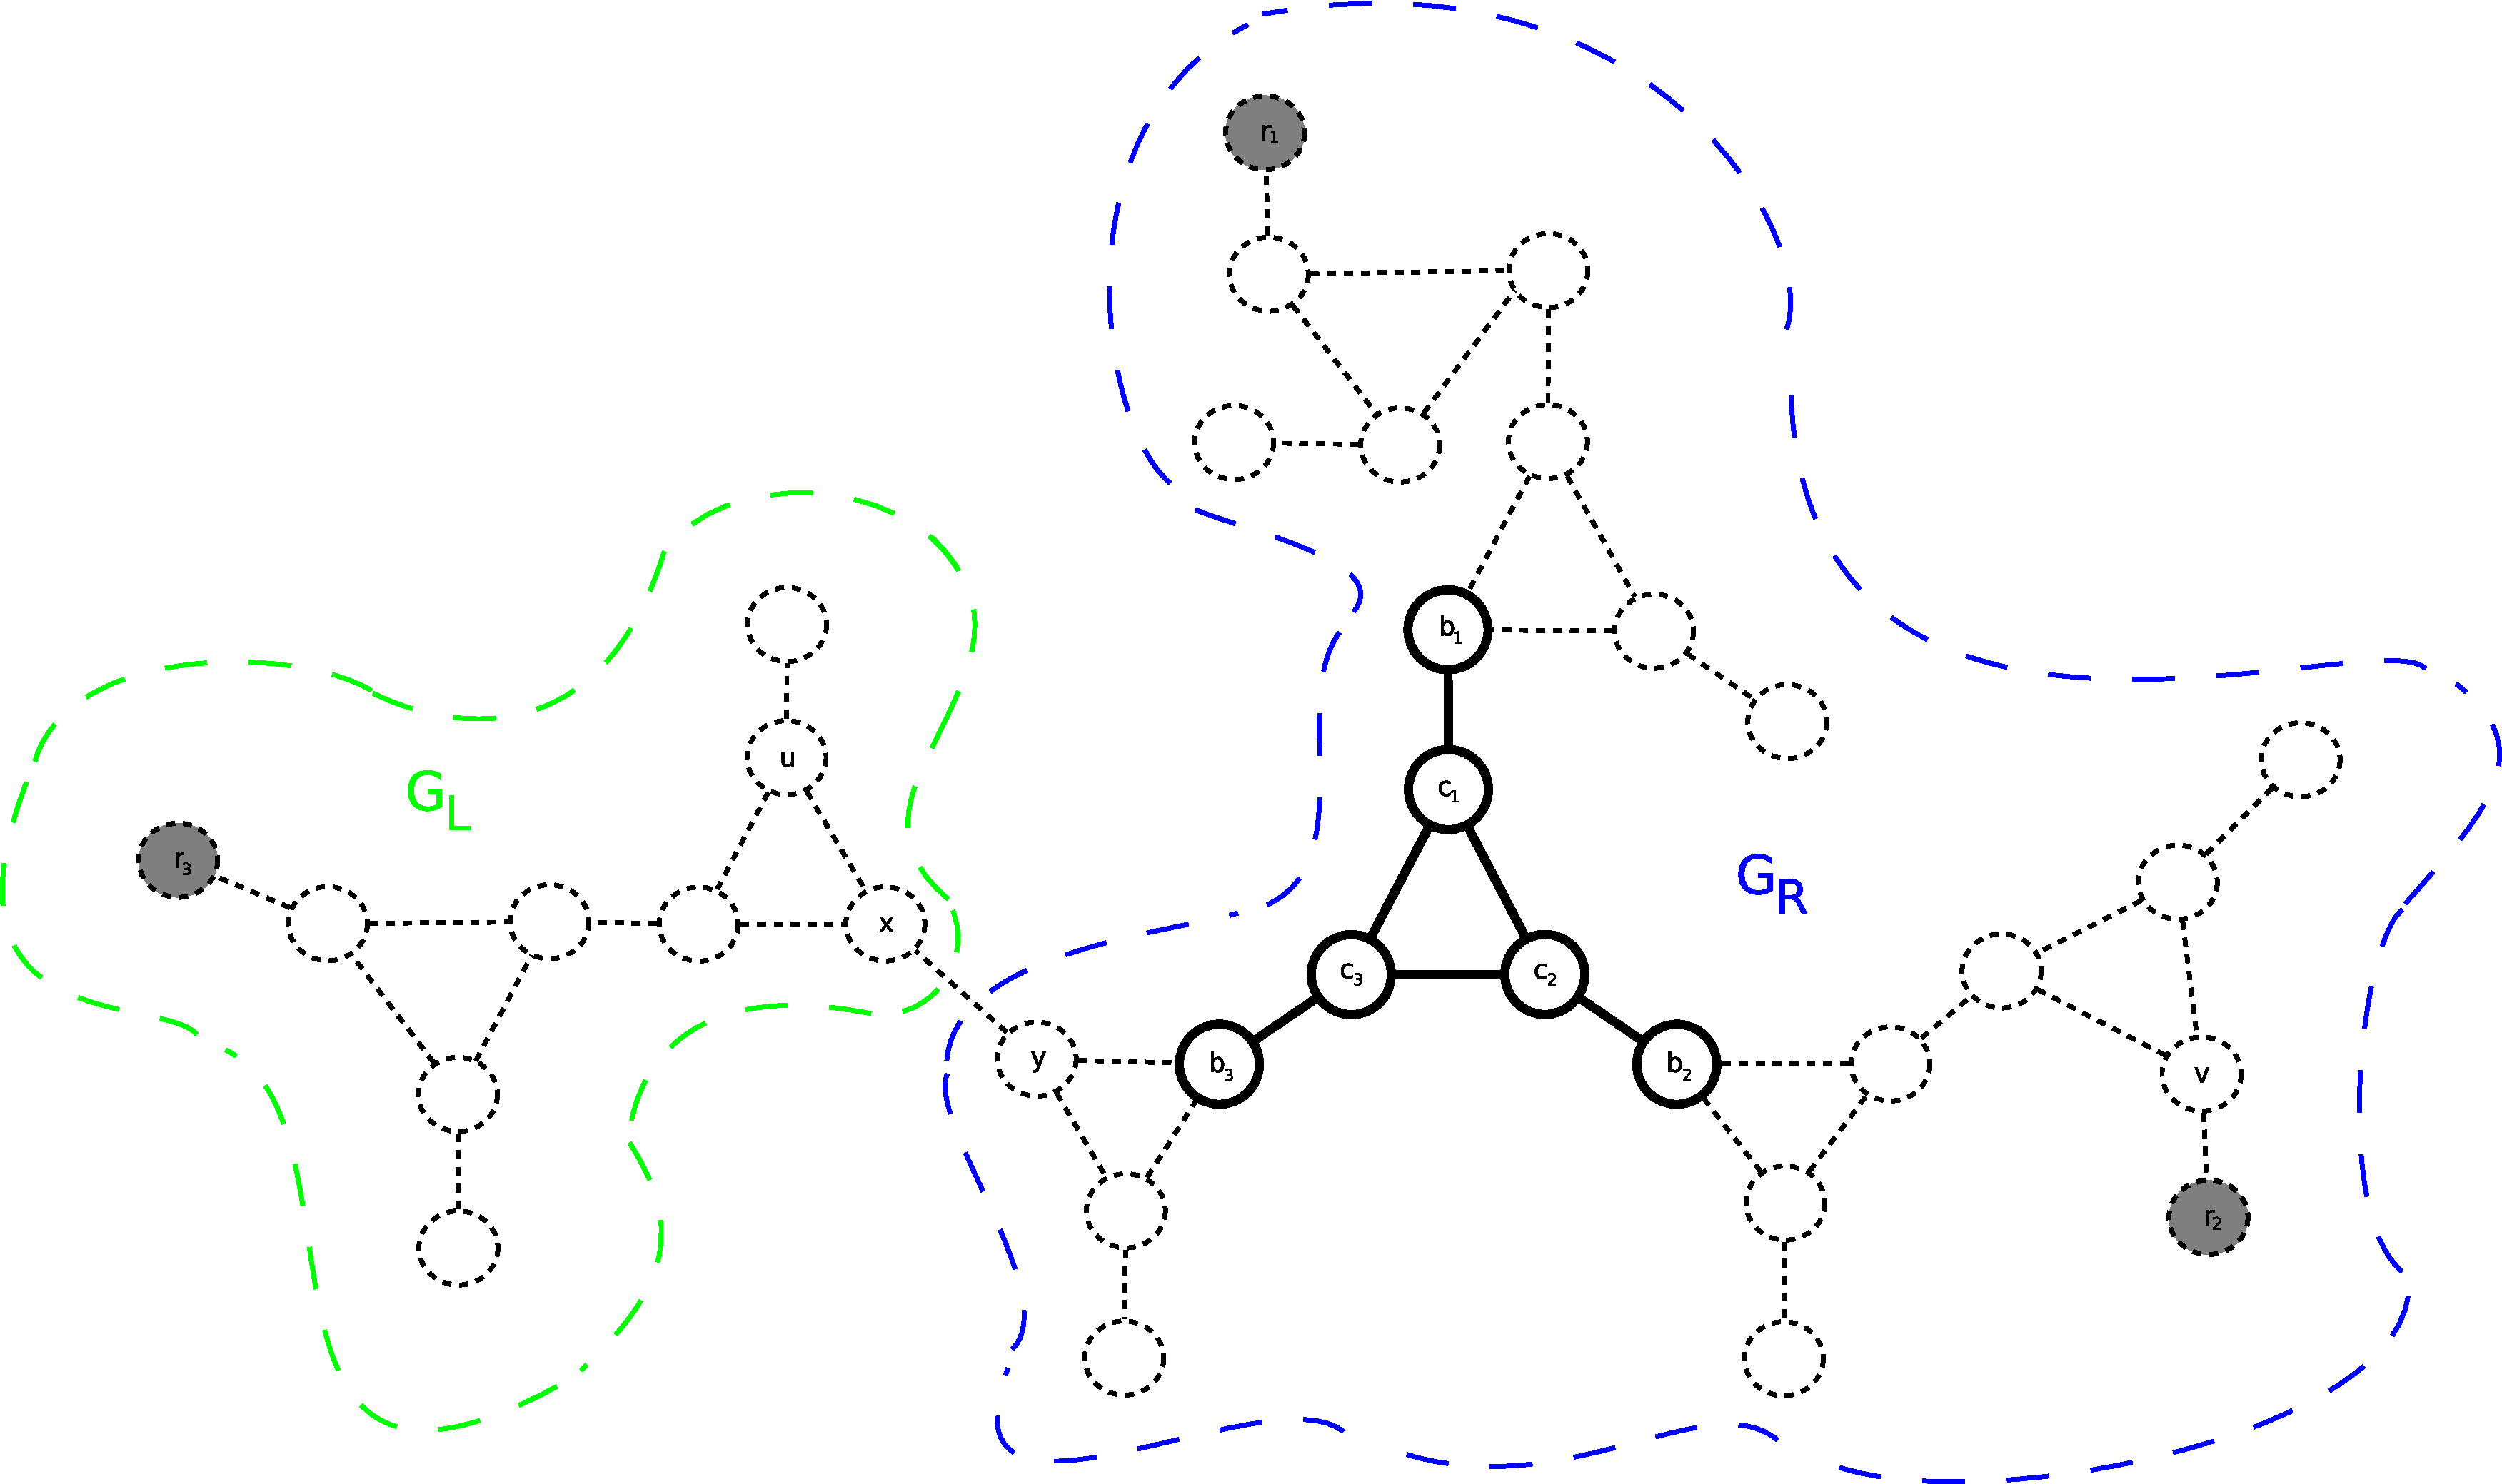
\includegraphics[width=380pt]{bew2.pdf}
   \caption{Ein Graph mit einem ausgesuchten $C_{3,j}$ und einem festen $r$}
  	 \end{figure}
  	 
\item Fall III. Die Knoten $u$ und $v$ haben die gleiche Distanz vom Knoten $r$ aus der metrischen Basis und die Knoten $u$ und $v$ liegen in unterschiedlichen $C_{3,j}$.\\
Durch die ursprünglichen Baumstruktur des Graphen gibt es zwischen den Knoten keine zwei knotendisjunkte Wege und insbesondere einen eindeutigen kürzesten Weg. Wie oben gibt es zu dem Knoten
\end{itemize}
\end{proof}
\begin{lem}
\textcolor{white}{x}
\begin{enumerate}
\item Fall: Der Baum besteht nur aus Knoten mit $deg(v) \leq 2$. Damit ist dieser Baum ein Weg und seine metrische Dimension ist eins.\\
\item Fall: Der Baum beinhalten genau einen Knoten mit $deg(v)=3$. Seine metrische Dimension ist zwei.
\end{enumerate}
\end{lem}
\newpage
\subsection{Verallgemeinerungen}
Unterschiedliche Möglichkeiten sind für die Verallgemeinerung von $C_j$-Bäumen möglich. Einerseits ist es möglich die Kreisordnung zu erhöhen. Eine andere Möglichkeit ist es jeden Knoten durch einen Kreis, welcher aus sovielen Knoten besteht wie der Grad des ersetzten Knotens, zu ersetzen und jeden Knoten eindeutig einem Nachbarn zuzuordnen. Man kann auch beide Arten vereinen und wie folgt definieren:
\begin{comment}
\begin{defi}
For a given tree $T=(V,E)$ with $deg(v_i)\leq 3$ for $v_i \in V$, the $C_j$ Tree is build in the following way: 
   Let $$V'=\{v_k|v_k \in V \wedge deg(v_k)=3\}\subseteq V$$ be a subset of the vertices of the graph $B$. Replace each element $v_j \in V'$ by a $C_k$ with $k \geq 3$ (call this subgraphs \emph{$C_{k,3,j}$}), so that at most one vertex of $C_{k,3,j}$ is connected to exactly one neightbour of $v_j$. The three neightbours of $C_{k,3,j}$ are called the \emph{$C_{k,3,j}$-$children$}. If two of the $C_{k,3,j}$-$children$ are leafs, so the subgraph including the $C_{k,3,j}$ his neighbours is called a \emph{$C_{k,3,j}$-$leaf$}.
\end{defi}

\begin{defi}
For a given tree $T=(V,E)$ with $deg(v_i)\leq n$ for $v_i \in V$, the $C_j$ Tree is build in the following way: 
   Let $$V'=\{v_k|v_k \in V \wedge deg(v_k)=n\}\subseteq V$$ be a subset of the vertices of the graph $B$. Replace each element $v_j \in V'$ by a $C_n$ (call this subgraphs \emph{$C_{n,j}$}), so that exactly one vertex of $C_{n,j}$ is connected to exactly one neightbour of $v_j$. The $n$ neightbours of $C_{n,j}$ are called the \emph{$C_{n,j}$-$children$}. If two of the $C_{n,j}$-$children$ are leafs, so the subgraph including the $C_{n,j}$ his neighbours is called a \emph{$C_{n,j}$-$leaf$}.
\end{defi}

\begin{defi}
For a given tree $T=(V,E)$ with $deg(v_i)\leq n$ for $v_i \in V$, the $C_j$ Tree is build in the following way: 
   Let $$V'=\{v_k|v_k \in V \wedge deg(v_k)=n\}\subseteq V$$ be a subset of the vertices of the graph $B$. Replace each element $v_j \in V'$ by a $C_k$ with $k \geq n$ (call this subgraphs \emph{$C_{k,n,j}$}), so that at most one vertex of $C_{k,n,j}$ is connected to exactly one neightbour of $v_j$. The t$n$ neightbours of $C_{k,n,j}$ are called the \emph{$C_{k,n,j}$-$children$}. If two of the $C_{k,n,j}$-$children$ are leafs, so the subgraph including the $C_{k,n,j}$ his neighbours is called a \emph{$C_{k,n,j}$-$leaf$}.
\end{defi}
\end{comment}
\begin{defi}
Sei ein Baum $T=(V,E)$ mit $deg(v_i)\leq n$ für $v_i \in V$ gegeben. Der $C_j$-$Baum$ resultiert daraus folgend: 
   Für alle $3 \leq i \leq n$ und $i \in \mathbb{N}$ sei $$V'=\{v_k|v_k \in V \wedge deg(v_k)=i\}\subseteq V$$ eine Teilmenge der Knoten aus dem Graphen $T$. Ersetze jedes Knoten $v_j \in V'$ durch einen $C_k$ mit $k \geq i$ (bezeichnet wird dieser Teilgraph als \emph{$C_{k,i,n,j}$}), so dass höchstens ein Knoten von $C_{k,i,n,j}$ mit genau einem Nachbarn von $v_j$ verbunden ist. Die $i$ Nachbarn von $C_{k,i,n,j}$ werden als \emph{$C_{k,i,n,j}$-$Kinder$} bezeichnet. Sofern zwei dieser $C_{k,i,n,j}$-$Kinder$ Blätter sind wird der Teilgraph, welcher den $C_{k,i,n,j}$ und seine Nachbarn beinhaltet, als \emph{$C_{k,i,n,j}$-$Blatt$} bezeichnet.
\end{defi}

\begin{satz}
\end{satz}
\subsection{Erweiterungen der Radgraphen $W_{1,i,n}$ und $W_{i,1,n}$}
\section{Metrische Dimension von außenplanaren Graphen% ist in $\mathbb{P}$
}
\todo[inline]{Alg. außenplanar} 

\section{Metrische Dimension von Halin Graphen}
\todo[inline]{Alg Halin Graphen}  
%%%%%%%%%%%%%%%%%%%%%%%%%%%%%%%%%%%%%%%%%%%%%%%%%%%%%%%%%%%%%%%%%%%%%%%%%%%%%%%%%%%%%%%%%%%%%%%%%%%%%%%%%%%%%%%%
%%%%%%%%%%%%%%%%%%%%%%%%%%%%%%%%%%%%%%%%%%%%%%%%%%%%%%%%%%%%%%%%%%%%%%%%%%%%%%%%%%%%%%%%%%%%%%%%%%%%%%%%%%%%%%%%
%%%%%%%%%%%%%%%%%%%%%%%%%%%%%%%%%%%%%%%%%%%%%%%%%%%%%%%%%%%%%%%%%%%%%%%%%%%%%%%%%%%%%%%%%%%%%%%%%%%%%%%%%%%%%%%%
\section{Zusammenfassung}
\begin{comment}
\begin{table}[htb]
\centering
 \renewcommand{\arraystretch}{1.5} 
\begin{tabular}{|l|c|c|c|c|c|}
\hline
$\:$Protocol & \multicolumn{1}{c|}{WSP} & GTSP & SP & SPP &SSP  \\
\hline
$\:$Cut $\&$ Choose & \Checkmark & \Checkmark  &\Checkmark & \Checkmark &  \XSolidBrush\\
\hline
$\:$Last-Diminisher & \Checkmark & (\Checkmark) & \Checkmark& \Checkmark &  \XSolidBrush\\
\hline
$\:$Lone-Chooser & \Checkmark & \Checkmark  &\Checkmark & \Checkmark &  \XSolidBrush\\
\hline
$\:$Lone-Divider & \Checkmark & \XSolidBrush  & \XSolidBrush &\XSolidBrush & \XSolidBrush \\
%\hline
%$\:$Cut your Own Piece & SPP & SP & \XSolidBrush & \Checkmark &SP& GSP \\
\hline
$\:$Divide-$\&$-Conquer & \Checkmark & \Checkmark &\Checkmark &\Checkmark &  \XSolidBrush \\
\hline
\end{tabular}
\caption{Overview: Strategyproofness of proportional cake-cutting protocols}\label{ov}
\end{table}
\end{comment}
%%%%%%%%%%%%%%%%%%%%%%%%%%%%%%%%%%%%%%%%%%%%%%%%%%%%%%%%%%%%%%%%%%%%%%%%%%%%%%%%%%%%%%%%%%%%%%%%%%%%%%%%%%%%%%%%
%%%%%%%%%%%%%%%%%%%%%%%%%%%%%%%%%%%%%%%%%%%%%%%%%%%%%%%%%%%%%%%%%%%%%%%%%%%%%%%%%%%%%%%%%%%%%%%%%%%%%%%%%%%%%%%%
%%%%%%%%%%%%%%%%%%%%%%%%%%%%%%%%%%%%%%%%%%%%%%%%%%%%%%%%%%%%%%%%%%%%%%%%%%%%%%%%%%%%%%%%%%%%%%%%%%%%%%%%%%%%%%%%
\subsection{Ähnliche Arbeiten}
\begin{comment}
\end{comment}
%%%%%%%%%%%%%%%%%%%%%%%%%%%%%%%%%%%%%%%%%%%%%%%%%%%%%%%%%%%%%%%%%%%%%%%%%%%%%%%%%%%%%%%%%%%%%%%%%%%%%%%%%%%%%%%%
%%%%%%%%%%%%%%%%%%%%%%%%%%%%%%%%%%%%%%%%%%%%%%%%%%%%%%%%%%%%%%%%%%%%%%%%%%%%%%%%%%%%%%%%%%%%%%%%%%%%%%%%%%%%%%%%
%%%%%%%%%%%%%%%%%%%%%%%%%%%%%%%%%%%%%%%%%%%%%%%%%%%%%%%%%%%%%%%%%%%%%%%%%%%%%%%%%%%%%%%%%%%%%%%%%%%%%%%%%%%%%%%%
\section{Offene Fragen und zukünftige Forschung}
\pagebreak

%%%%%%%%%%%%%%%%%%%%%%%%%%%%%%%%%%%%%%%%%%%%%%%%%%%%%%%%%%%%%%%%%%%%%%%%%%
%%%%%%%%%%%%%%%%%%%%%%%%%%%%%%% ENDE TEXTTEIL %%%%%%%%%%%%%%%%%%%%%%%%%%%%
%%%%%%%%%%%%%%%%%%%%%%%%%%%%%%%%%%%%%%%%%%%%%%%%%%%%%%%%%%%%%%%%%%%%%%%%%%

\clearpage
\thispagestyle{empty}
%\vspace*{\fill}g
\pagestyle{plain}
\bibliography{references.bib}
\bibliographystyle{apalike}
\thispagestyle{empty}
%\vspace*{\fill}g
\pagestyle{plain}
\clearpage

\listoffigures

\listoftables
\thispagestyle{empty}
%\pagebreak
\pagestyle{plain}
%\printindex
\end{document}
